% Minimalistic template for a generic article, geared towards MDPI guidelines
% Use PDFLaTeX
\documentclass[a4paper,10pt]{article}
% Packages provided by the MDPI template already
\usepackage[T1]{fontenc}
\usepackage[utf8]{inputenc}
\usepackage{lineno}
\usepackage{microtype}
\usepackage{amsmath}
\usepackage{indentfirst}
\usepackage{booktabs} % For \toprule, etc.
\usepackage[sort&compress,sectionbib]{natbib}
\bibliographystyle{newapa}

% Custom packages
\usepackage[acronym,toc,shortcuts,nohypertypes=acronym]{glossaries}
\usepackage[colorlinks, allcolors=blue, unicode]{hyperref}
\usepackage{hyperxmp} % Import license metadata
\usepackage{titling} % Get the author for the metadata
\usepackage{textcomp} % \texttimes
%\usepackage[pdf]{graphviz} % Importing dot files; can be replaced with generated PDFs
\usepackage[norefs,nocites]{refcheck} % Develop: warn if figure is not referenced

% Track changes package, remove when final; using a drop-in rather than the old version in TeX Live
% Usage: \added, \deleted, \replaced{new}{old}, \highlight, \comment
% All followed by an optional [id=<your id>, comment=<some comment>]
\usepackage[xcolor={usenames,dvipsnames}]{changes}
\definecolor{gem}{HTML}{003300}
\definechangesauthor[color=gem]{dm}
\definechangesauthor[color=NavyBlue]{jv}
\definechangesauthor[color=Purple]{nt}
\definechangesauthor[color=Mahogany]{mh}

% My own definition for the sections that start with a bold name but don't appear in TOC
\newcommand{\minisection}[1]{\medskip \textbf{#1:}}


% Metadata
\title{Fractional land cover classification method assessment using PROBA-V satellite data}
\author{Dainius Masiliūnas, Nandin-Erdene Tsendbazar, Martin Herold, \\ Myroslava Lesiv, Jan Verbesselt}
% * <Dainius Masiliūnas> 11:20:08 26 Mar 2019 UTC+0100:
% TODO: fix newline issue

\hypersetup{
    pdflicenseurl={http://creativecommons.org/licenses/by-sa/4.0/},
    pdfcopyright={This work is licensed under the Creative Commons Attribution-ShareAlike 4.0 International License.},
    pdfauthor={\theauthor}, % These are supposed to be the default but don't seem to be
    pdftitle={\thetitle},
    pdflang={en-GB}
}

% Acronyms - cite with \ac{}
\newacronym{GNSS}{GNSS}{Global Navigation Satellite System}
\newacronym{OA}{OA}{overall accuracy}
\newacronym{UA}{UA}{user accuracy}
\newacronym{PA}{PA}{producer accuracy}
\newacronym{RMSE}{RMSE}{root mean squared error}
\newacronym{MAE}{MAE}{mean absolute error}
\newacronym{ME}{ME}{mean error}
\newacronym{NSE}{NSE}{Nash–Sutcliffe model efficiency coefficient}
\newacronym{SDG}{SDG}{Sustainable Development Goal}
\newacronym{LC-CCI}{LC-CCI}{ESA Climate Change Initiative Land Cover}
\newacronym{CGLS}{CGLS-LC100}{Copernicus Global Land Services Land Cover}
\newacronym{FROM-GLC}{FROM-GLC10}{Finer Resolution Observation and Monitoring Global Land Cover}
\newacronym{SMA}{SMA}{spectral mixture analysis}
\newacronym{SVM}{SVM}{support vector machine}
\newacronym{MLP}{MLP}{multi-layer perceptron}
\newacronym{NN}{NN}{neural network}
\newacronym[text={random forest}]{RF}{RF}{random forest}
\makenoidxglossaries
% Disable abbreviating RF for now
\glsunset{RF}

% Use \begin{equation} for maths

\begin{document}

\maketitle

\linenumbers

\abstract{
\comment[id=dm]{The abstract is still a placeholder}The current common practice for producing global land cover maps is to represent land cover classes as discrete units, e.g. a pixel may be labelled as grassland, tree cover, or open water. However, in reality, the area covered by the pixel is hardly ever homogeneous, it may be e.g. trees surrounded by grass next to water. This mismatch between the reality and its representation in maps causes a loss in precision, as only the dominant land cover class can be represented in such ``hard'' classification maps. This problem is worse for coarse resolution land cover maps. A common workaround to this issue is to define mosaic classes, i.e. land cover classes that are combinations of other land cover classes, such as open forest (combination of grassland and tree cover). However, this approach leads to increasingly complex map legends and confusion about the definitions.

Our proposed solution to this issue is to employ fractional land cover mapping: for each pixel, define the proportion of the pixel that each considered land cover class occupies. This allows expressing an open forest as e.g. 40\% grassland, 60\% tree cover, and 0\% of the rest of the land cover classes. This ``fuzzy'' classification not only allows to more precisely express the land cover that exists in reality, but also gives users the flexibility to derive their own maps with a customised legend. For instance, if a user defines open forest as one that has less than 50\% tree cover and at least 30\% of grassland, they can generate a map with this definition from land cover fraction data, rather than relying on the definition that the mapmakers provide.
Exhaustive land cover fraction data is desired by a number of user communities, but to date there is no single global nor continental scale map that would provide fractions of each common land cover class.

In this paper, we tested the application of fractional land cover mapping over the continent of Africa. We compared the performance of four very different machine learning algorithms: random forest regression, multilayer perceptron neural networks, partial least squares regression, fuzzy nearest prototype classification and logistic regression. In order to allow the algorithms to make good predictions about land cover fractions, six types of covariates were used: spectral bands and vegetation indices derived from the Proba-V 100 m TOC reflectance data; temporal features derived from the full time series of said imagery; terrestrial features from a digital elevation model; soil properties and climate data from global models, and location. We compared the contribution of each of the covariate types to improving the accuracy of the model predictions.

One challenge when dealing with fractional data is the data imbalance: in most locations, only a single or a few classes dominate a pixel, with the rest taking up 0\% of the pixel. Values at the extremes (0\% and 100\%, i.e. pure pixels) are difficult for machine learning algorithms to estimate. We propose a new solution to this problem by combining three models: two classification models and one regression model. The first classification model determines whether a pixel is pure, and if so, it is processed using a classification model, otherwise it is processed with a regression model.

% Validation
% - 28k points
% - Independent training and validation sets

The models were trained on 26668 training points throughout Africa. The training points, collected as part of the Copernicus Global Land System: Dynamic Land Cover (CGLS-LC100) project, describe the fraction that each land cover class (bare soil, crops, grassland, shrubs, trees, urban/built-up, water and wetlands) occupies within a 100\texttimes100 m area, which is aligned to the grid used for Proba-V 100 m products. After the models were trained, their land cover class fraction predictions were compared with an independent validation set of 3617 points, which are likewise aligned to the Proba-V grid. Overall as well as per-class RMSE, MAE, and ME statistics were used to compare the models. In addition, the subpixel confusion-uncertainty matrix was used to analyse which classes were the most difficult to separate for each model, as well as to derive overall, users' and producers' accuracies and the kappa statistic. The models were compared with each other, as well as against a control intercept-only model.

Preliminary results show that the three-model approach increases the overall accuracy of the predictions by more accurately modelling the extreme values. From the machine learning models that were compared, random forest regression reaches the highest overall accuracy of 71\%. This is comparable to the reported accuracies of the current ``hard'' global land cover maps. Covariate importance analysis shows that spectral covariates are the most important for predicting land cover fractions, followed by the location, terrestrial and temporal covariates.

The application of the method on data gathered throughout Africa shows the applicability of the method to a variety of land cover conditions, ranging from highly heterogeneous agricultural landscapes to homogeneous bodies of water. Given enough reference data from other parts of the world and enough computational power, the method could be applied globally to upscale it to a global fractional land cover map. Such a map would cater to users with different fields of focus. Among other benefits, more precise estimation of land cover allows for 1) improved climate models to help reach Sustainable Development Goals (for which land cover is a key variable), 2) facilitate the making of models for vegetation and urban area dynamics, and 3) help governments and land owners keep better track of relevant land cover and its change. In addition, this work contributes to the operationalisation of the CGLS-LC100 project, which aims to produce exhaustive global land cover fractions as an operational product.

\minisection{Keywords} Fuzzy land cover classification, machine learning, random forest, gradient boosting, neural networks, fuzzy c-means, PROBA-V
}

\section{Introduction}
% * <Dainius Masiliūnas> 14:50:56 29 Jul 2019 UTC+0200:
% ~1250 words, 8 paragraphs + objectives

\begin{enumerate}
 \item Relevance of fractional LC mapping (link to user requirements and SDGs)
 \item Studies that have looked into fractional LC mapping so far
 \item Available fractional methods that were introduced in literature (wavelet transform etc.)
 \item Methods that are tested in this paper
 \item Global land cover maps
\end{enumerate}

Land cover, as one of the key variables for monitoring a number of \cglspl{SDG}, has received attention in recent years, and new global land cover maps have emerged to better map the current land cover of the world, as well as to track land cover change.
The most recent achievements have been the \ac{LC-CCI} map \highlight[id=dm, comment=Is there a better citation?]{\citep{defourny2012cci}} that aims at maintaining a long medium-resolution time series of global land cover for the climate community, \highlight[id=dm, comment=ditto]{\ac{CGLS}} map that aims at a finer spatial resolution and high quality with yearly updates since 2015, and the \ac{FROM-GLC} map \citep{fromglc2019} that showcases the potential of land cover mapping at 10 m resolution.

Most of these global land cover maps, as well as previous global land cover maps such as by \citet{bartholome2005glc2000, friedl2010modis, arino2007globcover, see2015hybrid, chen2015globeland30}, are provided as discrete classes (also known as ``hard'' or ``crisp'' classification), where each pixel of the map can only represent a single class.
However, this results in less precise estimation of land cover due to mixed pixels, where in reality there are multiple land cover classes in the area covered by a single pixel.
This issue becomes worse at coarse resolutions and heterogeneous landscapes.
It may result in biases, for instance, a sparse forest may be classified as grassland, ignoring the relatively few trees in the area, and thus ultimately lead to an underestimation of tree cover at large scales.

A potential solution to this issue is land cover fraction mapping, where instead of a discrete class, the proportion of every class in the legend is reported for every pixel of the map.
This is also called ``fuzzy'' or ``soft'' classification, and sometimes ``subpixel'' classification or ``linear mixture modelling'' \citep{Okeke2006fuzzyexponent}. A related term is ``super
Land cover fraction mapping has been attempted in the past, both in research \citep{adams_classification_1995, foody1996fuzzyevaluation, colditz_land_2011, sharma_assessing_2011, uma_shankar_wavelet-fuzzy_2011, dwivedi_optimisation_2012, lizarazo_quantitative_2012, gessner_estimating_2013, okujeni_generalizing_2018} and production (e.g. \citealp{hansen2000hardtree, hansen_continuous_2011, pengra_global_2015, hansen_global_2003, sexton_global_2013}).
Nevertheless, to date there is \highlight[id=dm, comment=Depends on how we position CGLOPS]{no global map} that would provide fractions of every major land cover class in a single product.

Land cover fraction mapping can be performed using different approaches and algorithms.
In its core, it is a regression rather than a classification problem, as the output is a fraction of a label rather than a label itself.
Popular approaches include fuzzy nearest centroid regression \citep{zhang2001fullyfuzzy}, \ac{SMA} (e.g. \citealp{yang_landsat_2012, hobbs2003linear, shimabukuro1991least}), \ac{RF} regression \citep{schwieder_estimating_2014}, \gls{SVM} regression \citep{schwieder_estimating_2014}, \gls{MLP} \glspl{NN} \citep{zhang2001fullyfuzzy}, genetic algorithms \citep{stavrakoudis_boosted_2011} and wavelet transformation \citep{uma_shankar_wavelet-fuzzy_2011}.



%The second drawback of current global land cover products is that their classification accuracy tends to be low, averaging at around 65\% \citep{tsendbazar2016integrating}. The third drawback is that all of these products use what is known as ``hard'' or ``crisp'' classification: each pixel is assigned to one particular land cover class only. The result of a hard classification is a thematic map. This classification type treats each pixel as homogeneous with regards to land cover, which is rarely the case in reality. In contrast, a ``fuzzy'' or ``soft'' classification, sometimes also called ``subpixel'' classification or ``linear mixture modelling'' \citep{Okeke2006fuzzyexponent} identifies the proportion of each land cover class within each pixel. The result of a fuzzy classification is one map per land cover class, showing the proportion of the pixel area covered by the land cover class.

%Hard classification is not well-suited for coarse resolution imagery, due to a large proportion of mixed pixels in it (representing areas of mixed land cover), compared to endmember pixels (or pure pixels, which are dominated by a single land cover class). When hard classification is attempted on such imagery, the accuracy of the result can be no higher than the area fraction that the dominant land cover type of the pixel occupies \citep{latifovic2004accuracy}. There have been attempts at increasing accuracy by defining mosaic classes, such as mixed forests (50\% needleleaf and 50\% broadleaf trees), but it leads to a proliferation of classes that increases map complexity and still does not deal with the core problem, thus not improving the classification accuracy by much \citep{tsendbazar2016comparative}. In contrast, ``fuzzy'' or ``soft'' classification results in each pixel containing information about the proportion of each class within that pixel, therefore operating on sub-pixel scales. This has the advantage of representing land cover more accurately, and gives the ability to represent mosaic classes as a combination of pure classes instead. Since the output of fuzzy classification is one raster per land cover class, with smooth transitions between classes, it is suitable for more in-depth analysis and user-specific visualisation criteria \citep{tsendbazar2016integrating}. Despite that, hard classification is still the most often used classification type due to the number of algorithms developed for it, ease of storing the result (it is thematic and thus takes little storage space), displaying it in a single map (albeit in a less accurate fashion) and performing accuracy assessment.

%There is a number of different classification algorithms, but only several of them are suitable to be used for fuzzy classification \citep{nath2014methods}. The two methods most commonly used in scientific literature are fuzzy \textit{c}-means and neural networks \citep{zhang2001fullyfuzzy}. Neural networks in particular are well-suited for fuzzy classification, since they allow multiple continuous output as well as input variables in a single model \citep{foody1997fuzzynnet}. Fuzzy \textit{c}-means, also known as fuzzy \textit{k}-means or soft \textit{k}-means, is a statistical method that relies on the proximity of pixels in feature space to class centroids, and thus is also suitable for fully fuzzy classification. However, since \textit{k}-means is an unsupervised classification algorithm, the ability to make use of training data in fuzzy \textit{c}-means is limited to determining class centroids with more precision \citep{hengl2004fuzzycmeans}.

%In addition, any other algorithms that provide a measure of uncertainty about class membership can be used, such as the ratio of individual tree votes of random forest \citep{breiman2001random} or class probabilities in gradient boosting \citep{friedman2001gradientboost}. While classification uncertainty is not a direct measure of class membership \citep{sytze2000fuzzyset}, they are nonetheless correlated. As such, it has been used by numerous authors as a proxy indicator of class membership, achieving satisfactory classification accuracy \citep{foody2002accuracy}.

%Furthermore, algorithms that can handle continuous variables, but only one response variable (such as random forest), can be used as well, by creating separate models for every class. This approach is called binary relevance \citep{karalas2016br}. Using this approach, the data needs to be post-processed after classification at a pixel level to conform to physical constraints (class membership must be between 0 and 100\% and sum up to 100\%). Random forest has been reported to give higher or equal accuracy results compared to other algorithms, like Support Vector Machines and individual decision trees, in hard classification scenarios using satellite imagery similar to that of PROBA-V \citep{duro2012algorithmcomparison}. Random forest regression was also shown to perform as well as other algorithms in fuzzy classification scenarios \citep{walton2008subpixelrf}, although it is used in much fewer studies on fuzzy classification than the other algorithms mentioned previously. Gradient boosting is an algorithm related to random forest, with the same advantages and disadvantages, but it is known to perform better in machine learning challenges \citep{chen2015higgs} and has not yet been tested on fuzzy land cover classification.

%Accuracy assessment is rather straight-forward for hard classification: typically a confusion matrix is employed for this purpose, showing how many pixels (or in some cases how much area \citep{stehman2009sampling}) in the image have been classified correctly, and how many incorrectly. Such a matrix makes it simple to tell which classes are hard to discern from one another, as well as allows for deriving statistics such as users' accuracy, producers' accuracy, and overall accuracy \citep{foody1996fuzzyevaluation}, as well as variance if probability sampling was used. However, a standard confusion matrix is not applicable in the context of fuzzy classification, since misclassification in this case is not absolute, but rather a matter of degree \citep{foody2002accuracy}. Several solutions, such as distance \citep{foody1996fuzzyevaluation}, cross-entropy and mutual information \citep{lu2007methods} have been suggested as alternatives for fuzzy classification accuracy assessment.

%Visualisation of the fuzzy classification results is also challenging, since each class effectively is a single-channel raster of its own. Three such classes can easily be combined into RGB channels for visualisation, but with more classes it is no longer possible. There have been attempts to develop a method based on the hue, saturation and intensity colour model to allow for a larger number of distinct classes to be visualised on a single raster \citep{hengl2004fuzzycmeans}. There is also a possibility of ``hardening'' the classification when high accuracy visualisation is not needed, and making use of multiple RGB rasters side-by-side when it is needed.

%All in all, even though global land cover mapping has been a focus of many other studies, existing global land cover maps still have room for improvement. This can be achieved by using data from the sensors of newer satellites such as PROBA-V, as well as performing fuzzy classification as opposed to the traditional hard classification.

%An important long-term goal of land cover mapping is to have a highly accurate fuzzy land cover classification method at a global scale. Since there are many different methods that could be used to achieve such a goal, and since the amount of data generated by satellites covering the entire world is enormous, this thesis focuses on comparing several different fuzzy classification methods on a subset of global imagery provided by the PROBA-V satellite.

%PROBA-V is a relatively new satellite, with few studies using it for land cover classification so far. A number of studies have used simulated PROBA-V data in preparation for its launch \citep{stathakis2014probavurban,roumenina2013probavcrops,bartalev2014probavboreal}. After launch, most studies have focused on its potential for crop classification \citep{roumenina2015probavcrops,durgun2016crop,lambert2016cropland}. All of these studies have only used the traditional hard classification. As such, the potential of using PROBA-V data for fuzzy classification in order to obtain a more accurate representation of land cover at global scale has never been tested before.

%Another problem of land cover classification is that there is high disagreement between different land cover products on mixed classes, such as mixed forests \citep{Herold2008lccomparison}. Mixed forests and wetlands are challenging to detect and classify using hard classification and optical remote sensing data, so it is important to check how well large-scale fuzzy classification performs on these classes. Therefore this thesis focused specifically on the region of ecotone from boreal forests to temperate broadleaf forests in Europe. This region also includes a large number of boreal wetlands. 

%In addition, there is a wide variety of methods that can be used for fuzzy classification. Most studies on this topic focus on comparing only two methods at once. In this thesis, four of them have been tested: fuzzy \textit{c}-means, neural networks, random forest regression and multiclass gradient boosting. All of these methods are based on fundamentally different approaches to classification, so the results give insight into the possible performance of similar methods as well. In addition, the last of the mentioned methods has not yet been tested on fuzzy classification itself (although related methods have been).

%When it comes to global image processing, one problem is the amount of data and the time it takes to process it. Some algorithms are known to suffer from the curse of dimensionality, where a linear increase in input data results in a geometric increase in processing time \citep{walton2008subpixelrf}. Therefore it is important to also measure the processing time of different classification methods.

In addition to classification methods, one aspect that is important for classification accuracy is the data (covariates) that the algorithm is trained on and predict land cover from \citep{yu2014metadiscoveries}. In addition to spectral covariates (blue, red, near infrared, shortwave infrared bands), temporal covariates (growing season start, duration, growing intensity) are commonly used to improve the separability of crops \citep{jakubauskas2001harmonic}. Elevation covariates (elevation, slope, aspect) are known to improve the separability between tree classes \citep{burrough2001fuzzy}. Vegetation indices have been used to improve the detection of wetlands \citep{sader1995wetlands}, as well as for defining classification rules in rule-based fuzzy classification \citep{baraldi2006rulebased}. Therefore in this thesis such covariates have also been used in order to increase land cover classification accuracy, and their importance for prediction was analysed.

\textbf{Objectives}:

\begin{enumerate}
 \item Compare the performance of a variety of machine learning models for a global-scale land cover fraction mapping task
 \item Compare the importance of covariates and covariate groups for the prediction of land cover fractions
 \item Investigate methods for reducing bias in the predictions with regards to zero inflation and predictions tending towards the mean
\end{enumerate}


\section{Data and Methods}

\subsection{Reference data}

For training the global land cover fraction models, a training dataset collected by IIASA was used. This global point dataset provides information on nine class fractions of sampled pixels of the Proba-V 100 m product.
The fraction estimate was acquired by high-resolution image interpretation by regional experts, for the year 2015.
Each of the sampled Proba-V pixels was subdivided into a 10-by-10 subpixel grid and the area estimates were derived from the subpixel ratios.

For model validation, an independent global dataset collected by Wageningen University \& Research was used.
The method of point collection is equivalent to the method used for training data collection, but performed by separate teams of regional experts.

The data includes over 150\,000 training points and over 20\,000 validation points across the globe (see figure \ref{fig-reference-data}).
Since the data describes fractions, it is zero-inflated, since it is relatively rare for more than just a few land cover classes to occupy a single pixel; the rest are set to zero.

\begin{figure}
 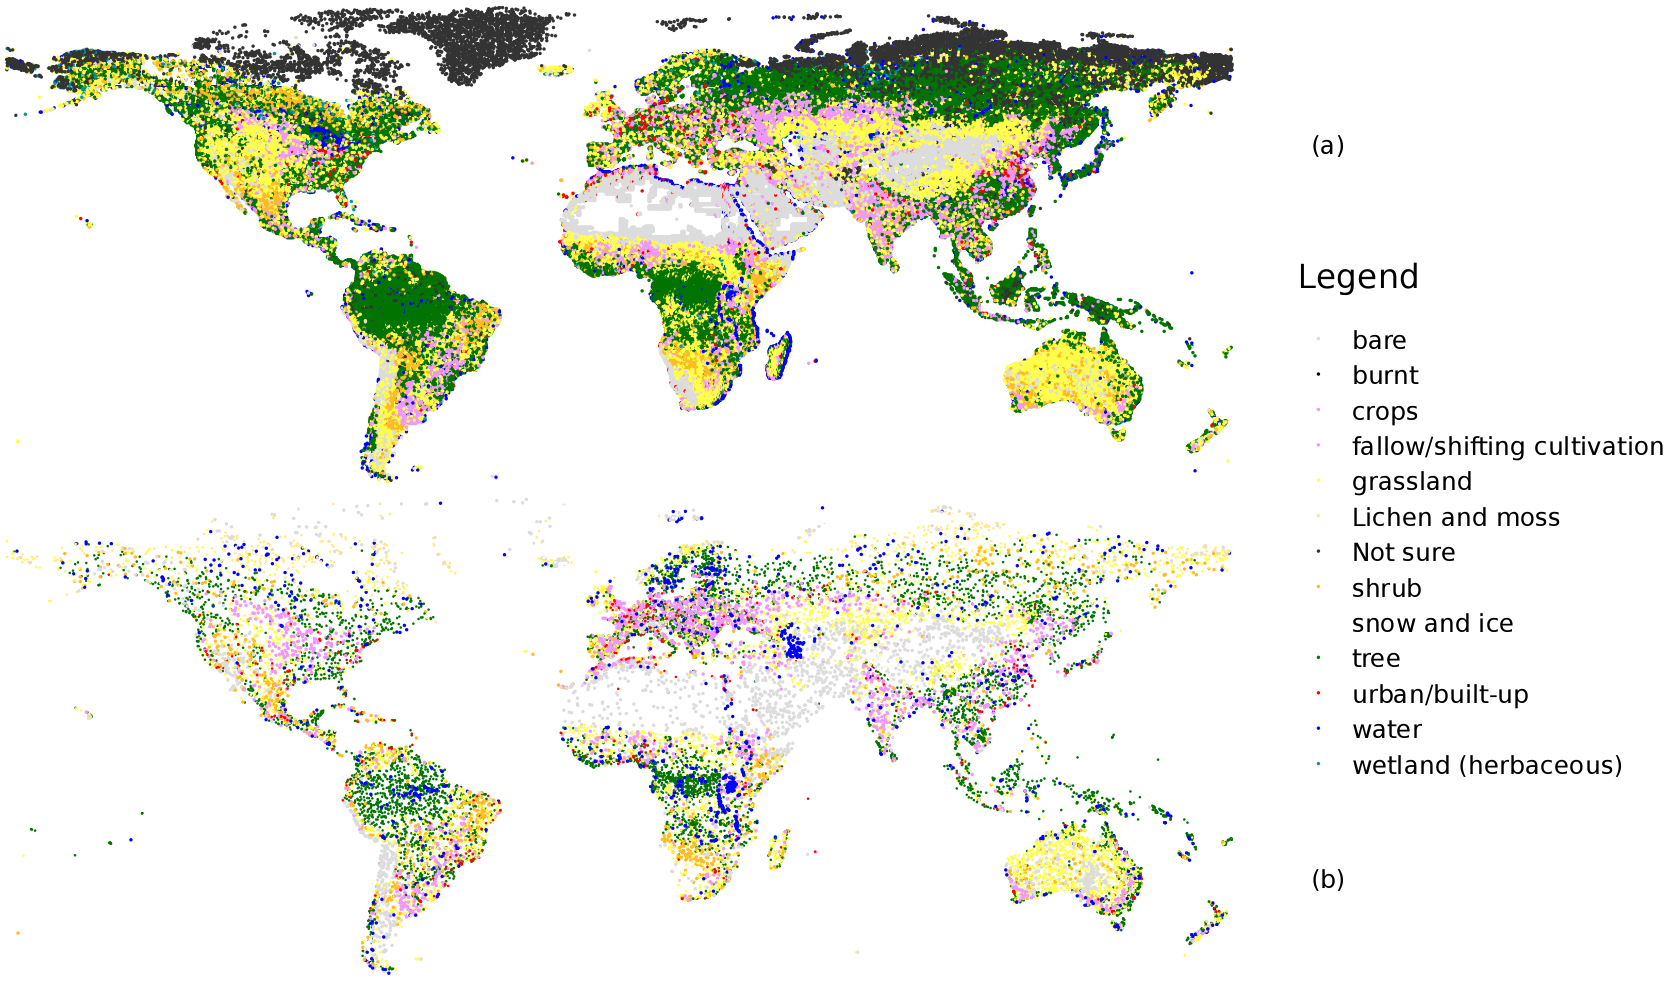
\includegraphics[width=\textwidth]{article-figures/maps/2019-08-06-training-and-validation}
 \caption{Reference data points with the dominant land cover class. (a): training dataset. (b): reference dataset.}
 \label{fig-reference-data}
\end{figure}

\subsection{Model covariates}

To predict land cover fractions in unsampled areas, the models learn from covariates present at the locations of the training data, and then the covariates are used for prediction in unsampled areas.
In this study, five groups of covariates were used: optical, terrain, soil, climate and location.
All of these covariates had to be preprocessed before they could be input into the models.

\subsubsection{Optical covariates}

\begin{figure}
 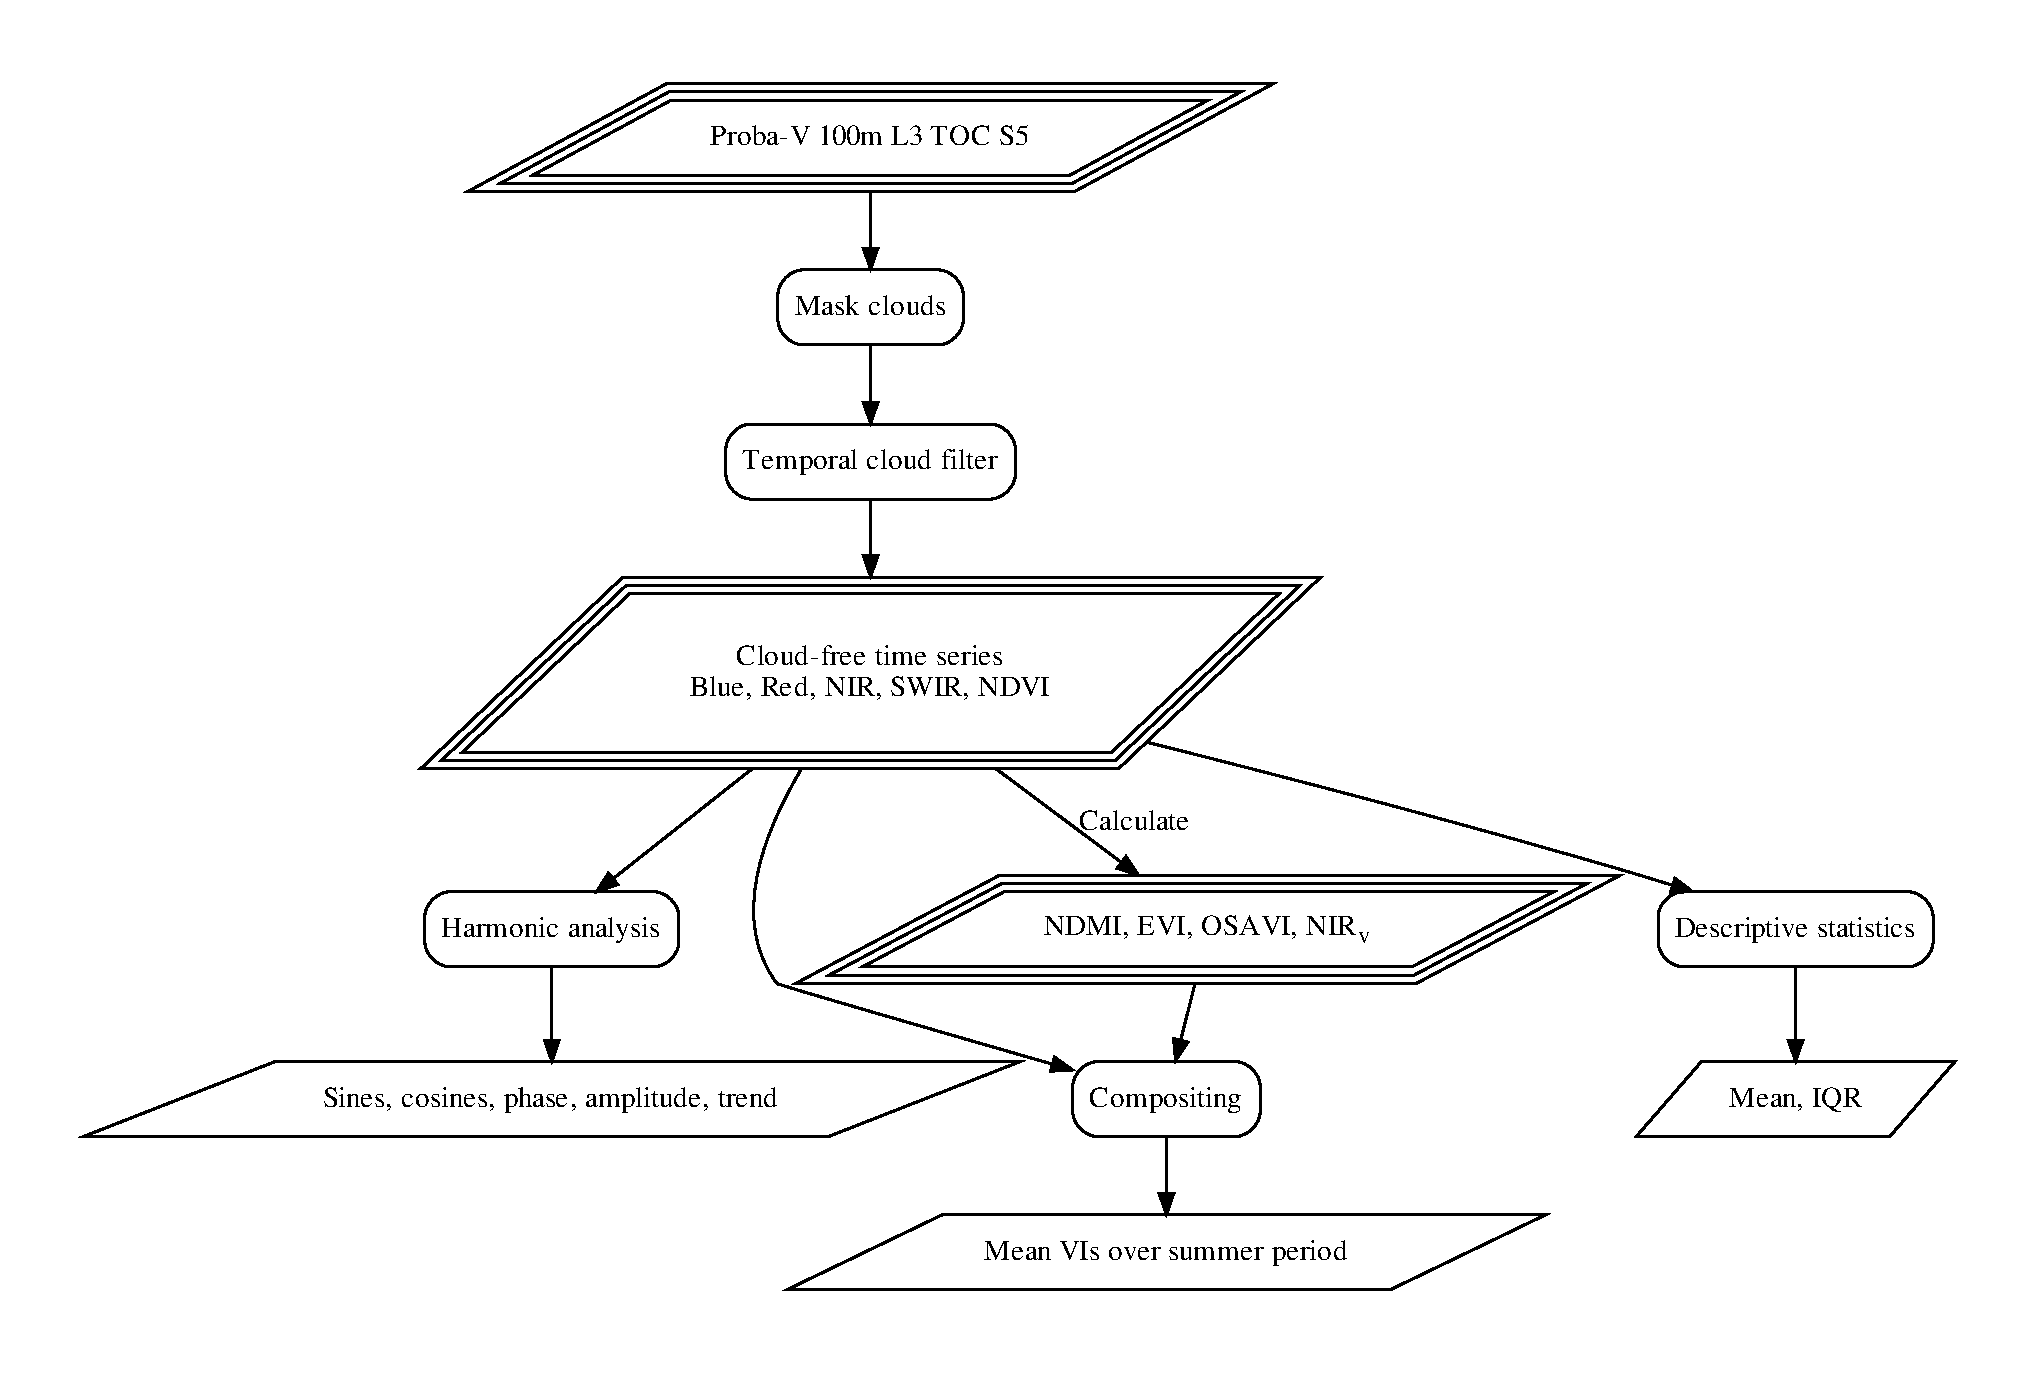
\includegraphics[width=\textwidth]{article-figures/flowcharts/preprocessing-optical}
 \caption{Optical data preprocessing chain.}
 \label{fig-preprocessing-optical}
\end{figure}

\begin{enumerate}
 \item GLSDEM
 \item Proba-V time series
 \item SoilGrids and LandGIS
 \item WorldClim
\end{enumerate}

\subsection{Preprocessing}

\begin{enumerate}
 \item Temporal cloud filter for Proba-V
 \item Harmonic metrics extraction
 \item Terrain metrics calculation
 \item Additional climate parameter calculation
 \item Manual model feature selection
\end{enumerate}

%\begin{figure}
 %\inputdigraph[width=\textwidth]{article-figures/algorithms}{dot}
% 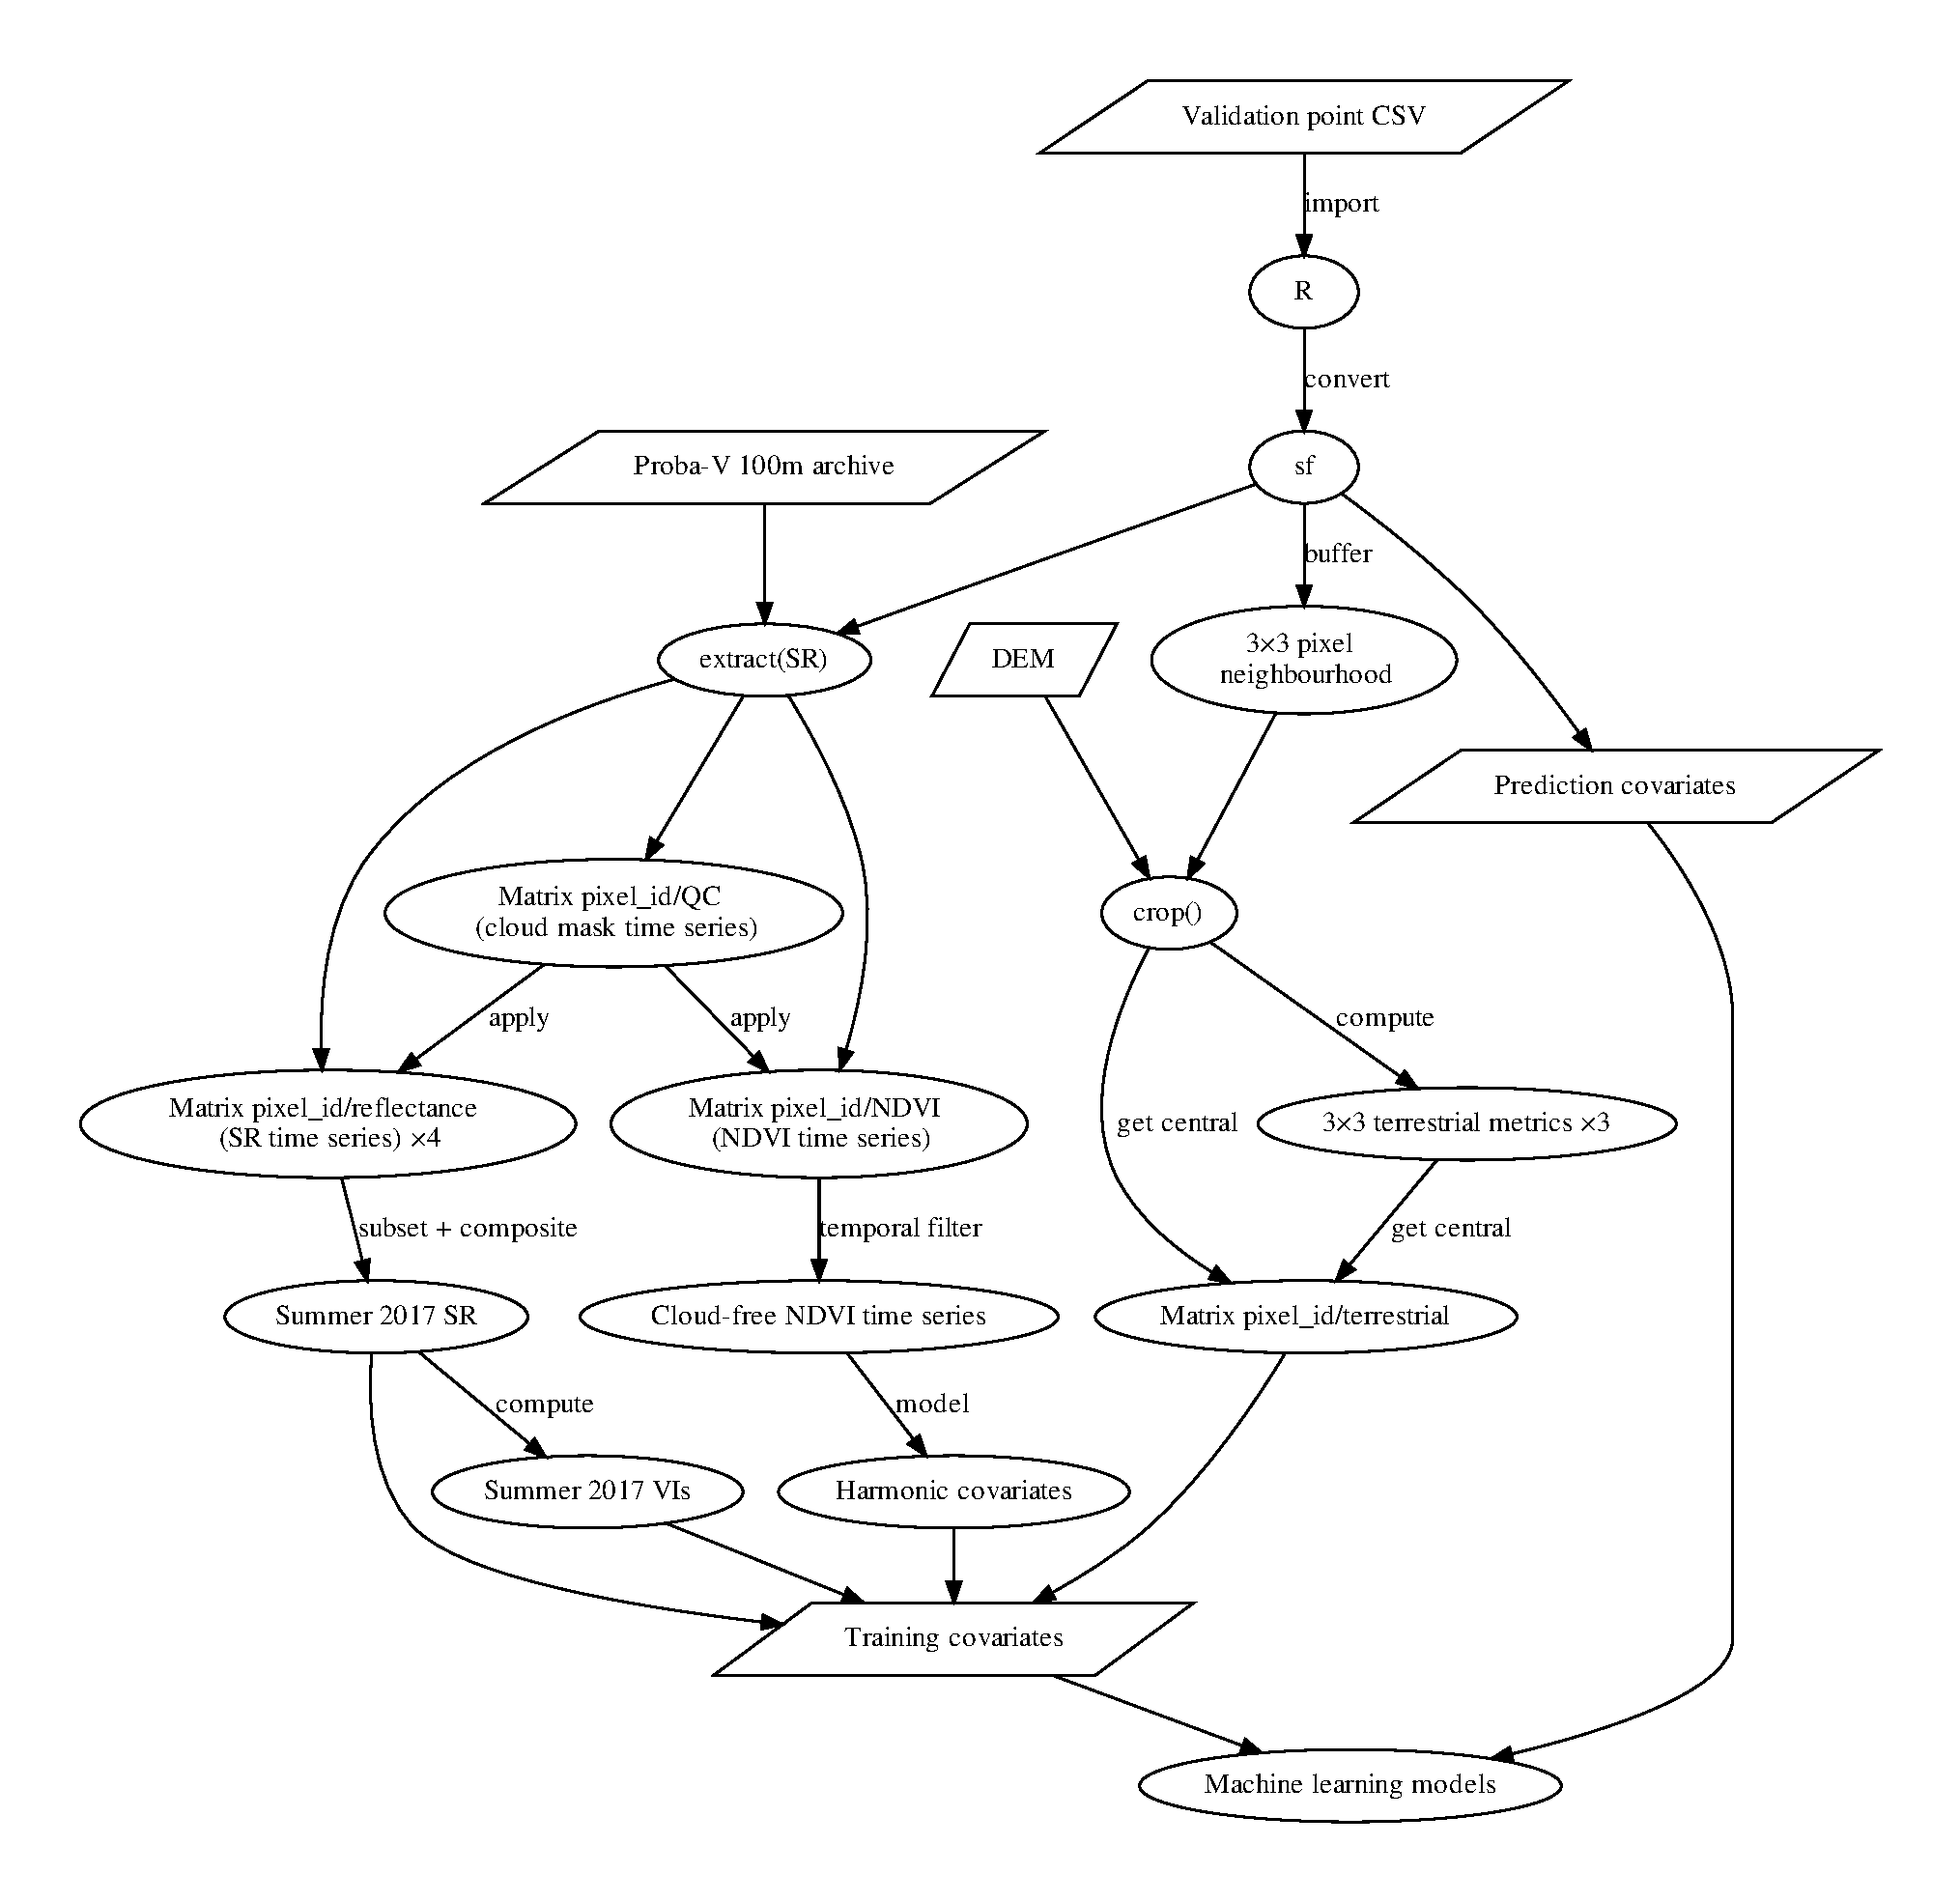
\includegraphics[width=\textwidth]{article-figures/flowcharts/algorithms}
% \caption{Preprocessing chain.}
% \label{fig-preprocessing}
%\end{figure}

\begin{figure}
 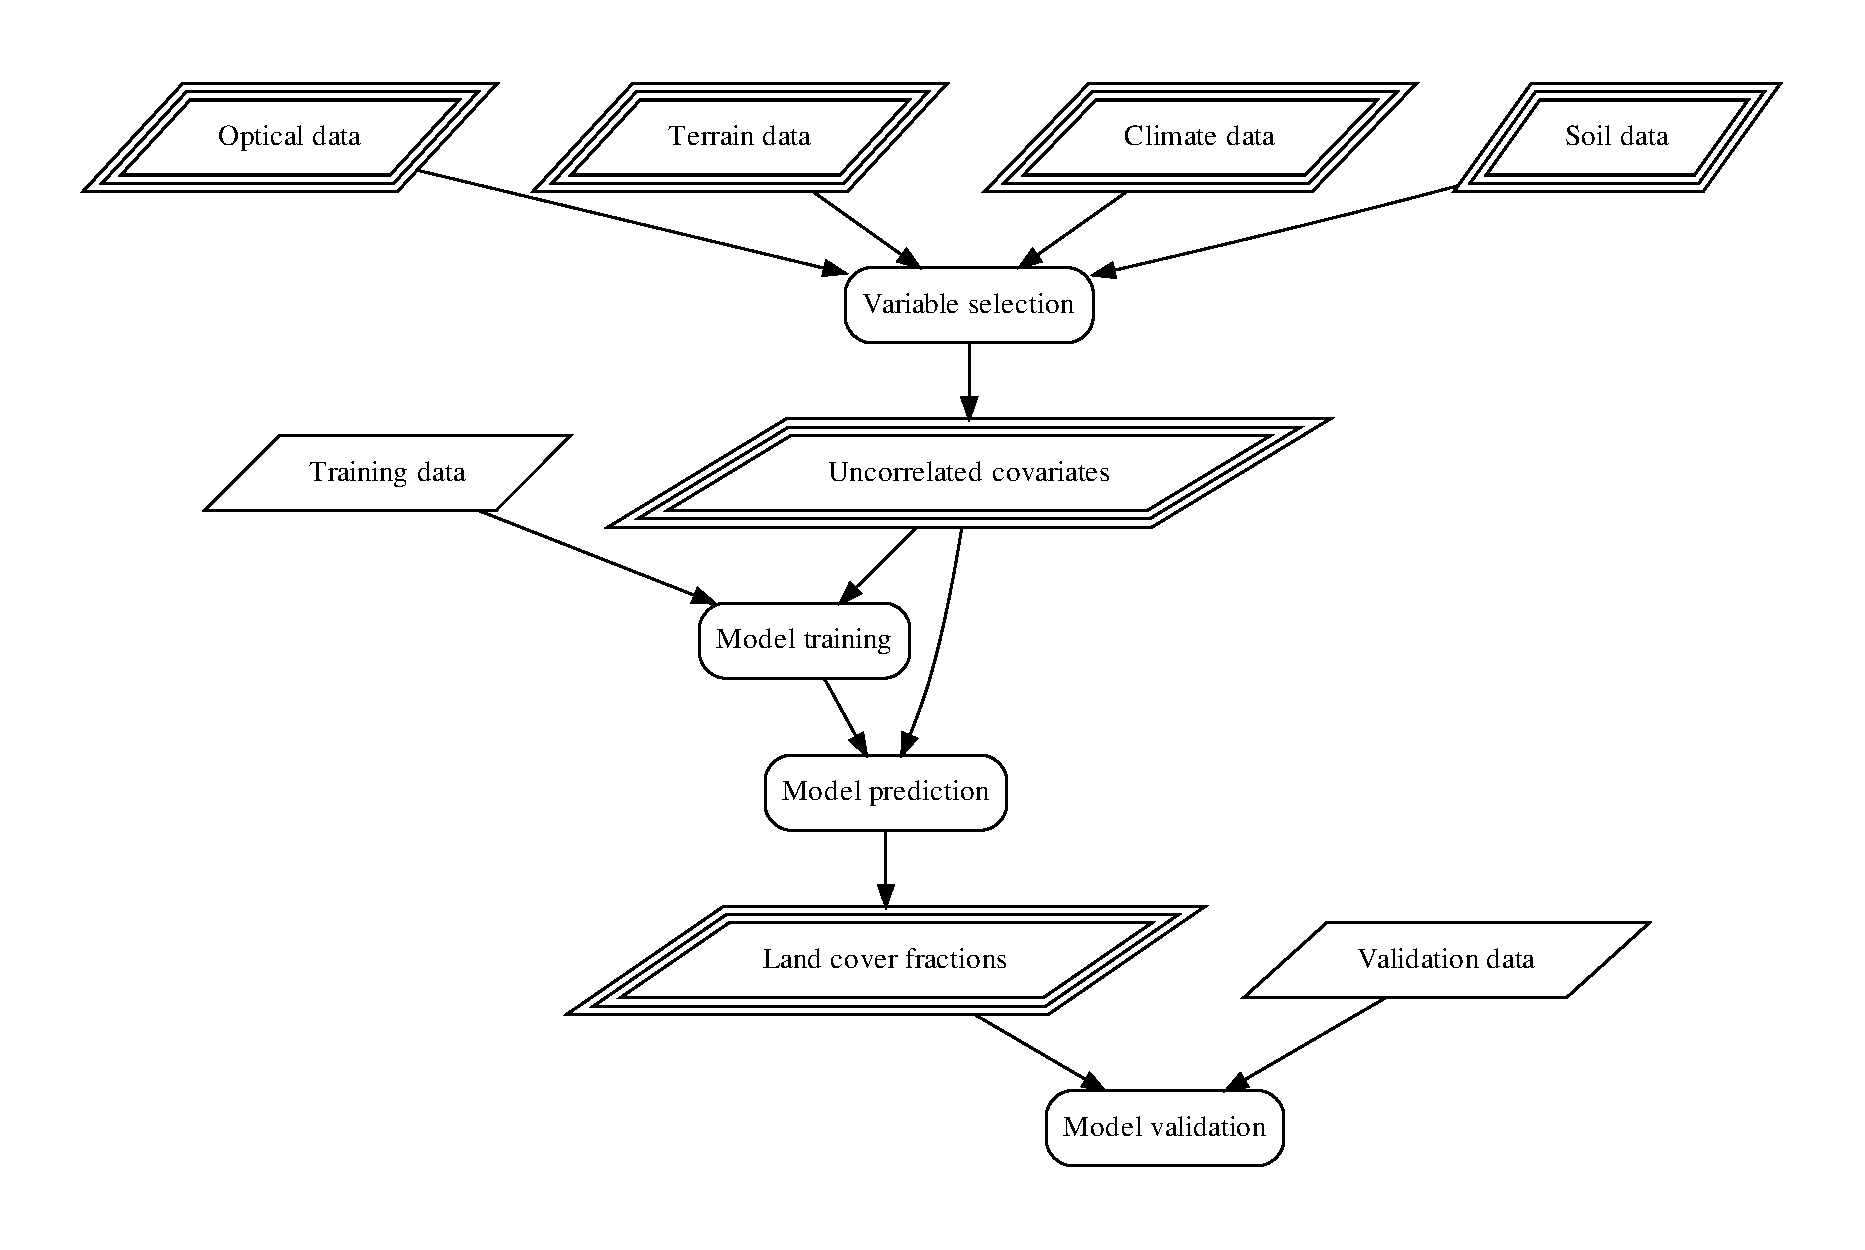
\includegraphics[width=\textwidth]{article-figures/flowcharts/processing}
 \caption{Processing chain.}
 \label{fig-processing}
\end{figure}

\subsection{Fractional land cover mapping methods}

\subsubsection{Logistic regression}

\subsubsection{Lasso/ridge/elastic net regression}

\subsubsection{Partial least squares regression}

\subsubsection{Fuzzy nearest prototype/centroid}

\subsubsection{Neural networks}

AKA multilayer perceptron

\subsubsection{Random forest regression}

Including variable importance

\subsection{Model tuning (multi-step approach) to account for value imbalance}

As the dataset is unbalanced (dominated by zeroes and hundreds) and thus the objective function tends to draw the model towards good prediction of 0/100, whereas in regression the middle is also important. Therefore we tried several approaches to increase the accuracy of the middle predictions.

We compared a single model of the best algorithm, to a two-step approach: one model to predict zeroes, and one model to predict non-zeroes; and a three-step approach, with one model to predict pixel purity (i.e. if we face a classification or a regression problem), one to perform regression (on mixed pixels) and one to perform classification (on pure pixels).

In addition, we investigated applying histogram matching, by matching the histogram of the predictions back to the histogram of the training set.

\subsection{Validation/Accuracy Assessment}

Not sure if this should be a section, or just part of results:

\begin{enumerate}
 \item \ac{RMSE}, \ac{MAE}, \ac{ME} per class
 \item Sub-pixel confusion-uncertainty matrix: kappa, \ac{OA}, \ac{PA}, \ac{UA}
 \item Correlation matrix
 \item Prediction accuracy at different parts of the predicted vs observed line
 \item Comparison with a control/intercept model (10\% of everything)?
\end{enumerate}

\section{Results}

\begin{enumerate}
 \item RMSE per class comparison: no big differences
 \item Subpixel confusion matrix metrics: quite a big difference
 \item RF variable importance
 \item Truth:prediction scatterplots (hex/box/bar)
 \item Point map of Africa for the different classes
\end{enumerate}

\subsection{Method accuracy comparison}

The intercept model (always predicting the mean) achieves an \ac{RMSE} of 30\%, and \ac{OA}

Logistic regression achieved RMSE of 18.7\%, MAE of 9.8\%, 

\begin{table}
\centering
\begin{tabular}{llllll}
\toprule
\textbf{Model} & \textbf{\ac{RMSE} (\%)} & \textbf{\ac{MAE} (\%)} & \textbf{\acrshort{NSE}} & \textbf{\ac{OA} (\%)} & \textbf{Kappa} \\
\midrule
Intercept
& 30.7  & 21.8  & 0     & 24±4  & 0.11±0.04 \\
Fuzzy nearest centroid
& 22    &       &       & 49    & 0.41      \\
Neural networks
& 19.5  &       &       &       &           \\
PLS regression
& 19    &       &       & 47±5  & 0.36±0.07 \\
Logistic regression
& 20.0  & 10.7  & 0.53  & 66±4  & 0.57      \\
Lasso regression
& 18.5  &       &       &       &           \\
Random forest
& 16.6  & 9.2   & 0.67  & 68±4  & 0.60      \\
\ensuremath{''} histogram matched
& 22.0  & 9.7   & 0.43  & 66±2  & 0.58±0.03 \\
\ensuremath{''} two-step
& 18.3  & 8.0   & 0.59  & 72±2  & 0.63      \\
\ensuremath{''} three-step
& 18.6  & 8.2   & 0.59  & 71±4  & 0.64      \\
\ensuremath{''} \ensuremath{''} histogram matched
& 21.3  & 9.1   & 0.46  & 68±3  & 0.61      \\
\bottomrule
\end{tabular}
\caption{Accuracy statistics of the models tested.}
\label{tab-accuracy}
\end{table}

% 1:1 plots
\begin{figure}
    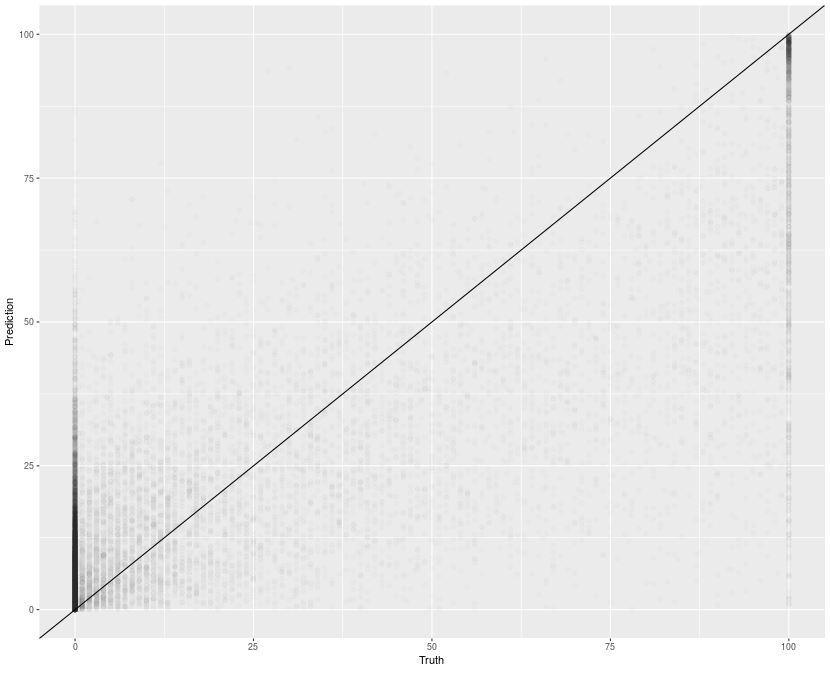
\includegraphics[width=0.8\textwidth]{article-figures/binplots/2019-04-12-rf-1m-uncor-points-a001s2}
    \caption{Random Forest single model prediction correspondence to ground truth (raw points with overplotting).}
    \label{raw-rf-1m-uncor}
\end{figure}
% Binplots
\begin{figure}
    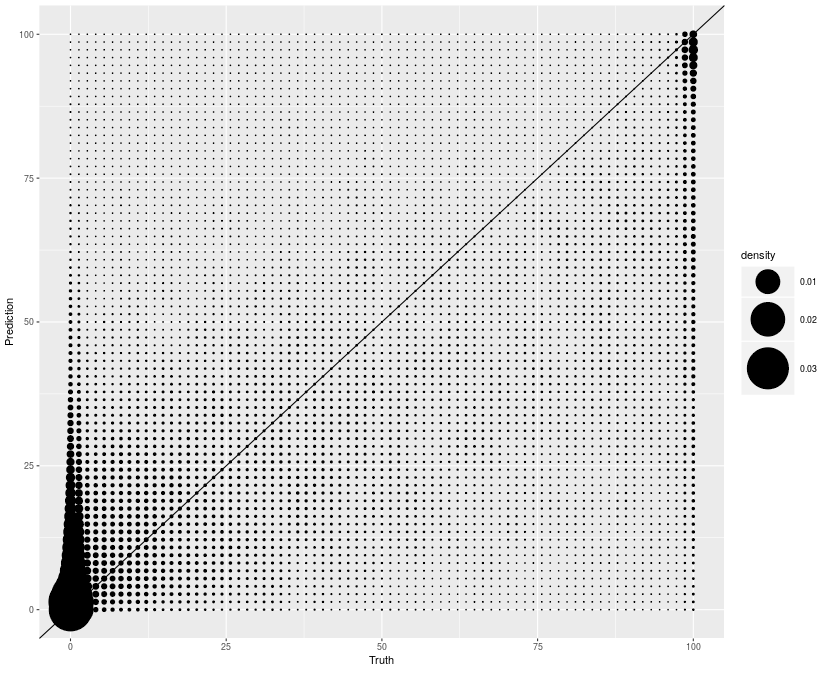
\includegraphics[width=0.8\textwidth]{article-figures/binplots/2019-04-12-rf-1m-uncor-point-n100s20}
    \caption{Random Forest single model prediction correspondence to ground truth, 100x100 bins.}
    \label{bin-rf-1m-uncor-n100}
\end{figure}
\begin{figure}
    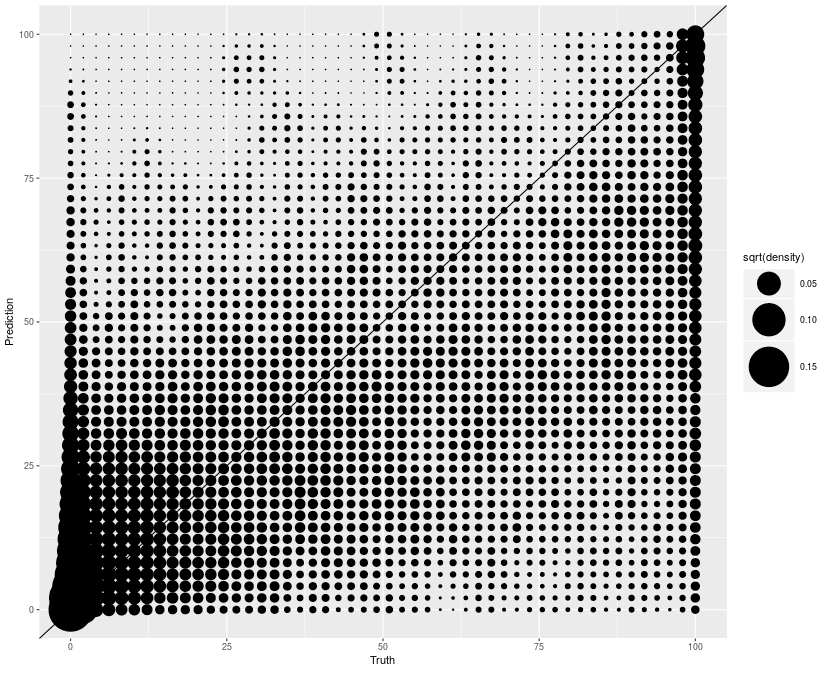
\includegraphics[width=0.8\textwidth]{article-figures/binplots/2019-04-12-rf-1m-uncor-point-n50s20sqrt}
    \caption{Random Forest single model prediction correspondence to ground truth, 50x50 bins, square root transformation.}
    \label{bin-rf-1m-uncor-n50sqrt}
\end{figure}
\begin{figure}
    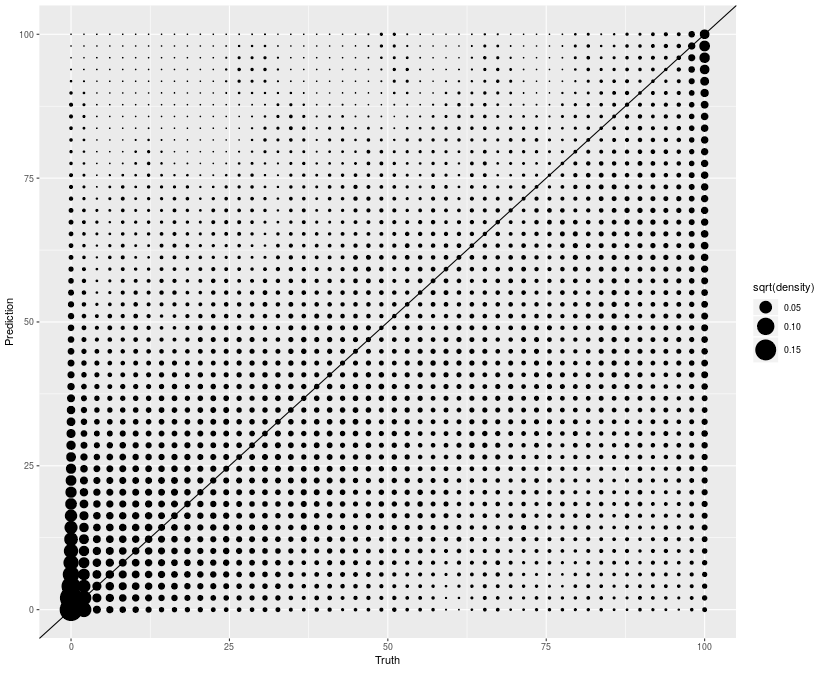
\includegraphics[width=0.8\textwidth]{article-figures/binplots/2019-04-12-rf-1m-uncor-point-n50s10sqrt}
    \caption{Random Forest single model prediction correspondence to ground truth, 50x50 bins, square root transformation, smaller circle sizes.}
    \label{bin-rf-1m-uncor-n50sqrts10}
\end{figure}
\begin{figure}
    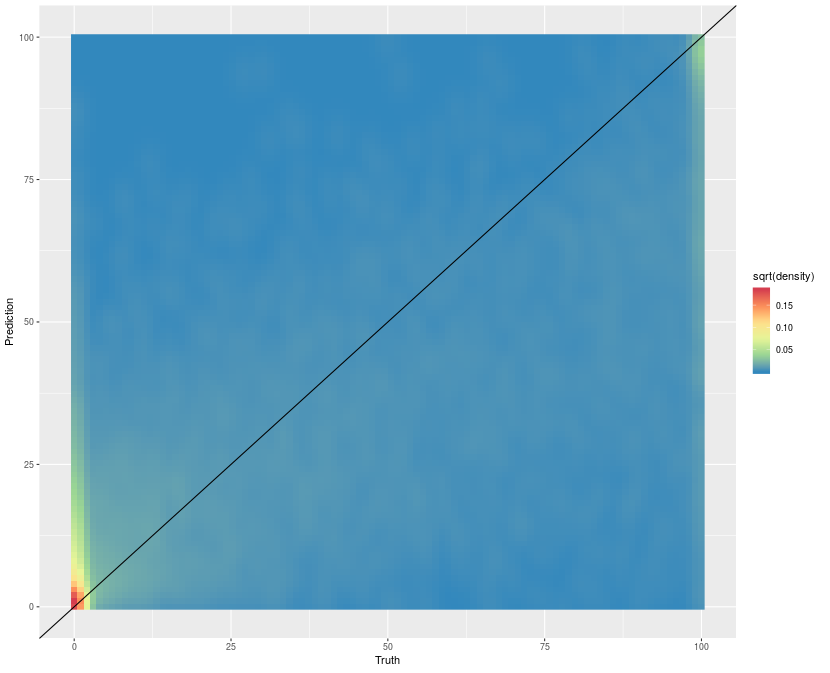
\includegraphics[width=0.8\textwidth]{article-figures/binplots/2019-04-12-rf-1m-uncor-raster-n50sqrt}
    \caption{Random Forest single model prediction correspondence to ground truth, square root transformation.}
    \label{bin-rf-1m-uncor-rastersqrt}
\end{figure}

% Hexplots
\begin{figure}
    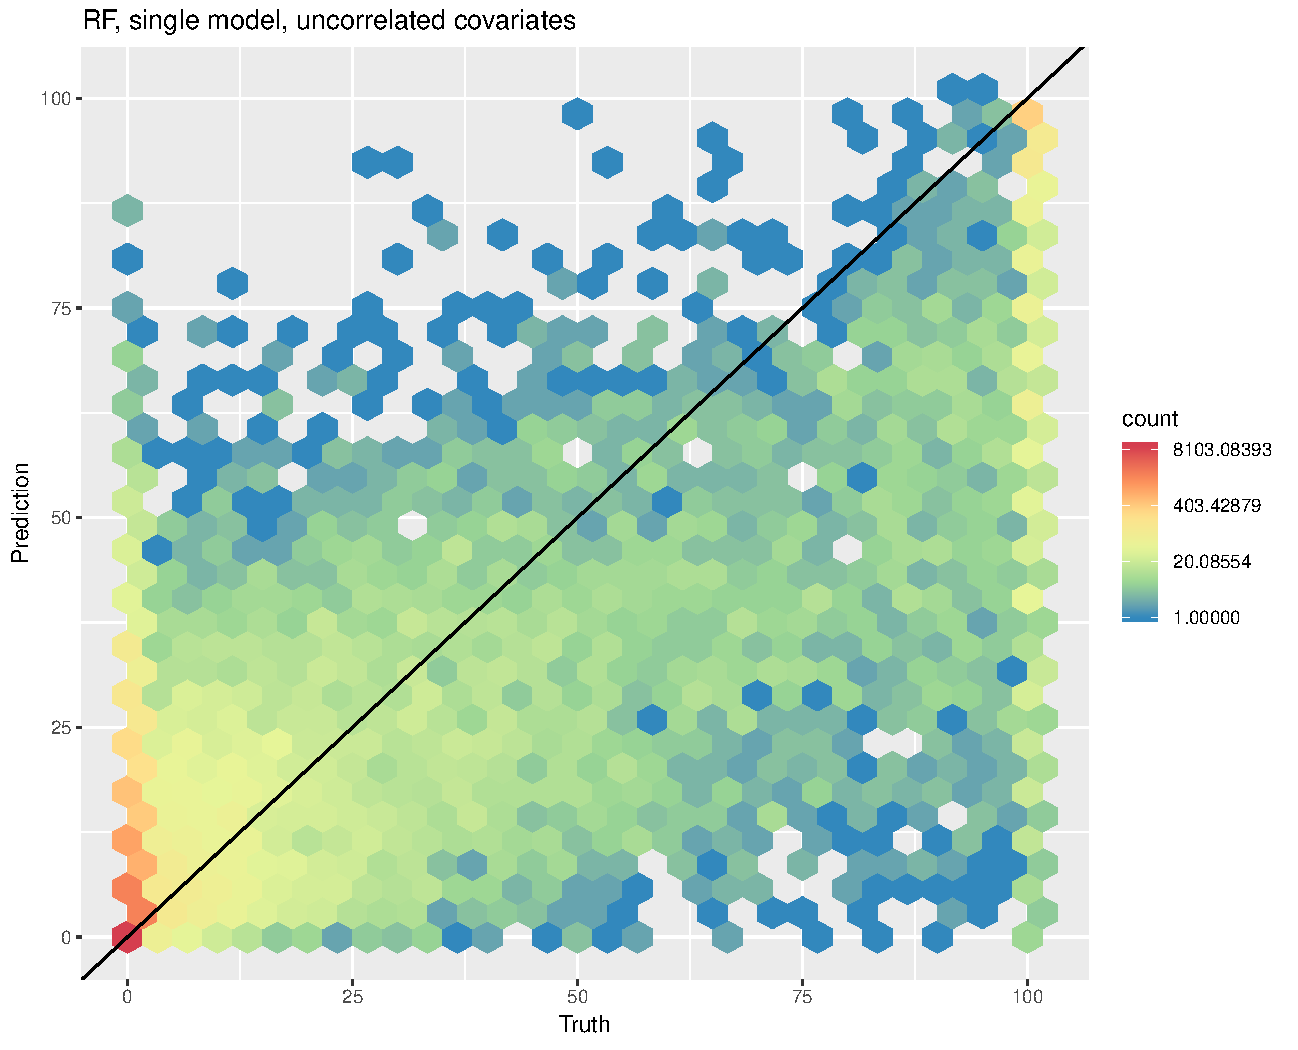
\includegraphics[width=0.8\textwidth]{article-figures/hexplots/2019-03-22-rf-1m-uncor-hex}
    \caption{Random Forest single model prediction correspondence to ground truth.}
    \label{hex-rf-1m-uncor}
\end{figure}
\begin{figure}
    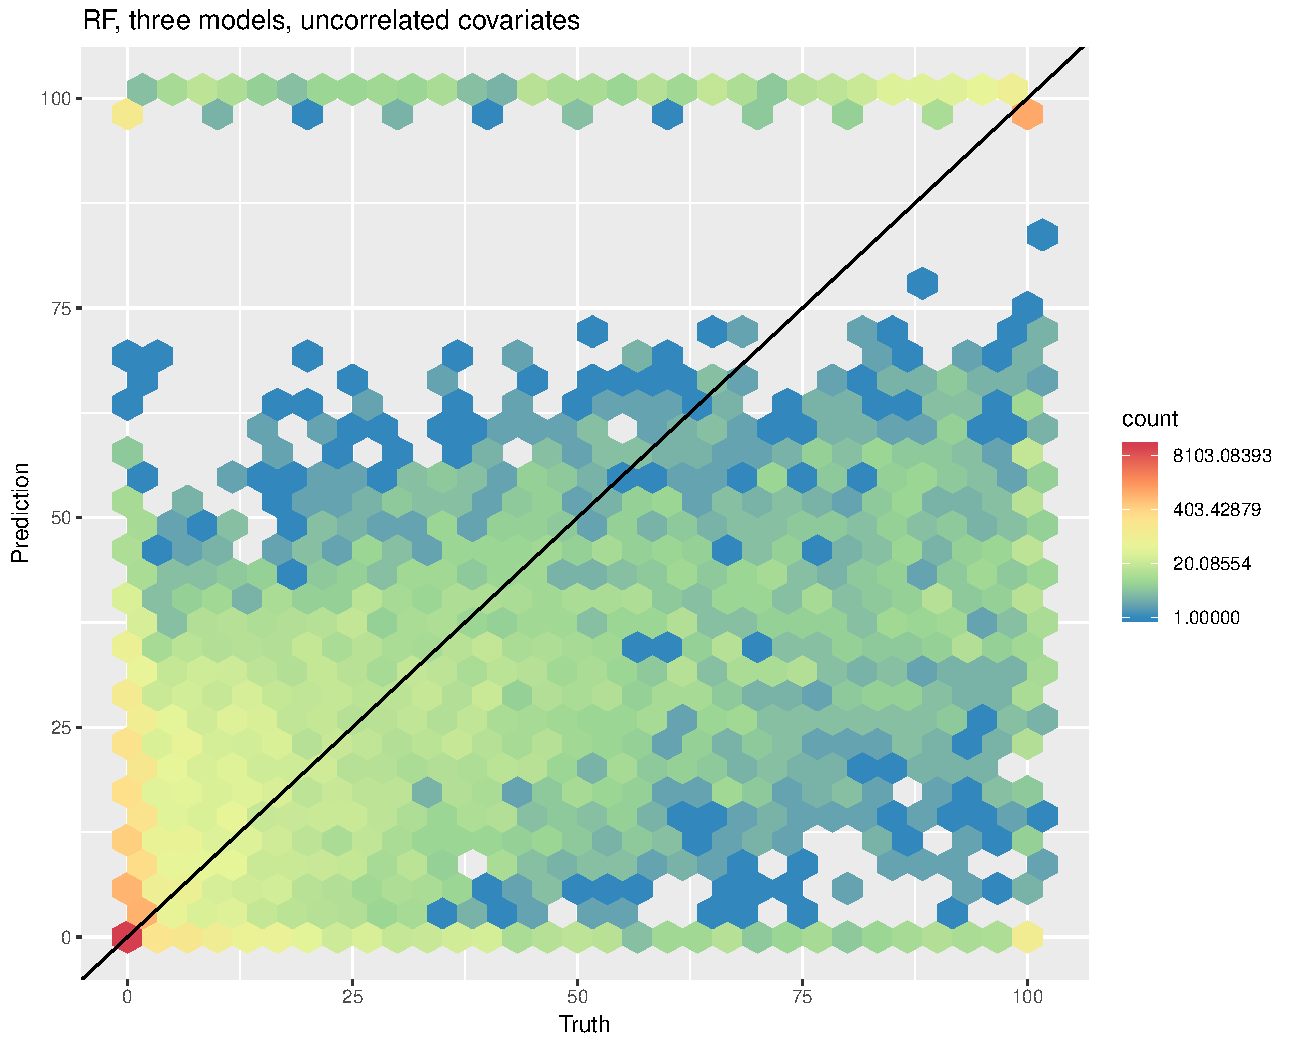
\includegraphics[width=0.8\textwidth]{article-figures/hexplots/2019-03-22-rf-3m-uncor-hex}
    \caption{Random Forest three-step model prediction correspondence to ground truth.}
    \label{hex-rf-3m-uncor}
\end{figure}
\begin{figure}
    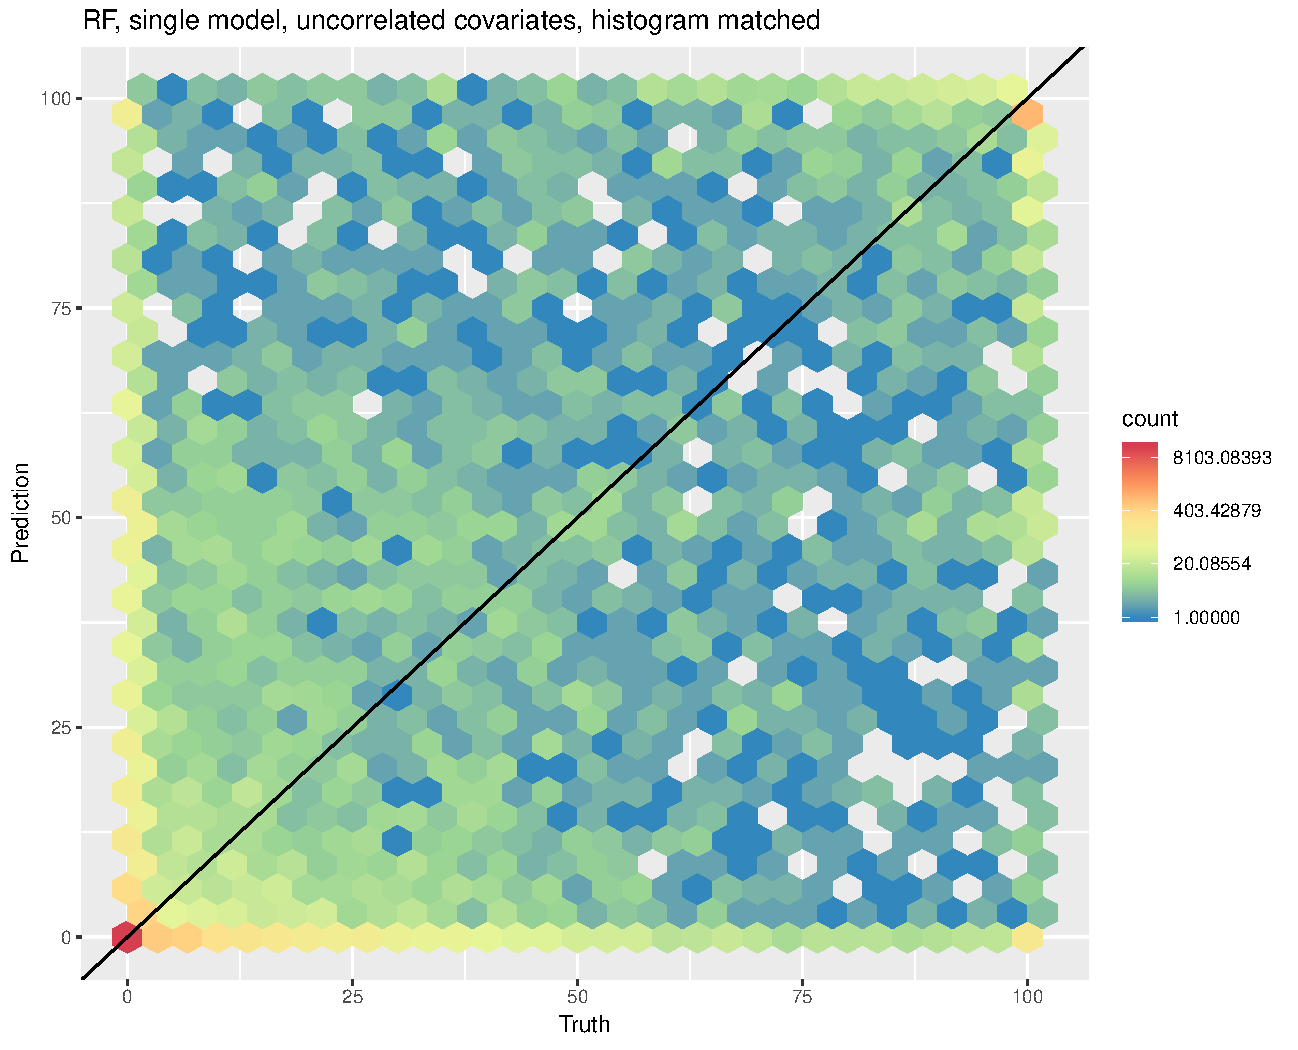
\includegraphics[width=0.8\textwidth]{article-figures/hexplots/2019-03-22-rf-1m-uncor-hm-hex}
    \caption{Random Forest single model prediction (histogram matched) correspondence to ground truth.}
    \label{hex-rf-1m-uncor-hm}
\end{figure}
\begin{figure}
    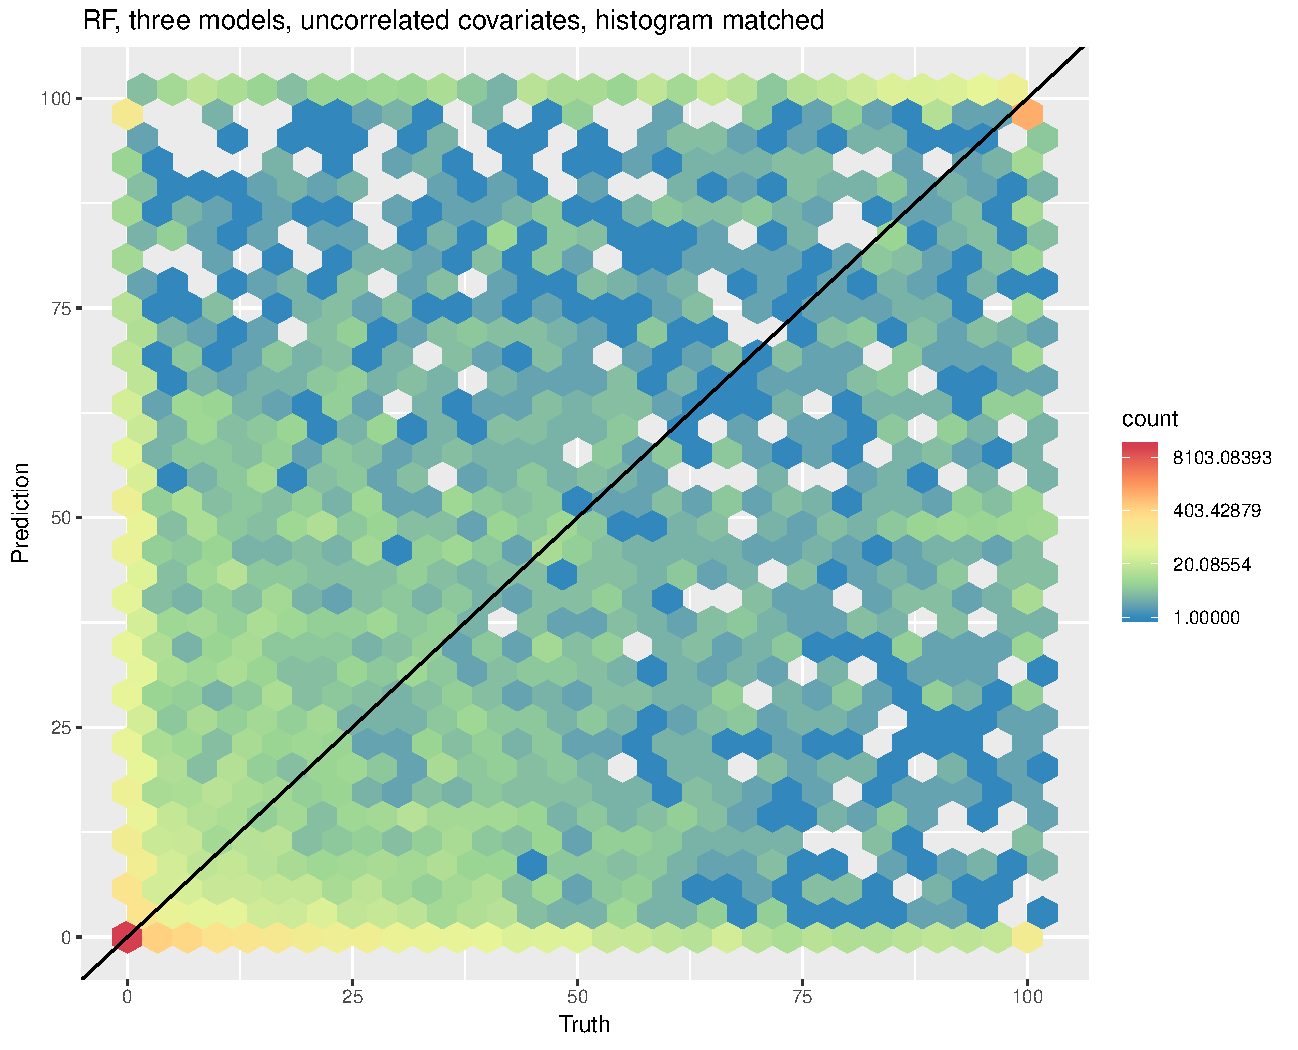
\includegraphics[width=0.8\textwidth]{article-figures/hexplots/2019-03-22-rf-3m-uncor-hm-hex}
    \caption{Random Forest three-step model prediction (histogram matched) correspondence to ground truth.}
    \label{hex-rf-3m-uncor-hm}
\end{figure}
\begin{figure}
    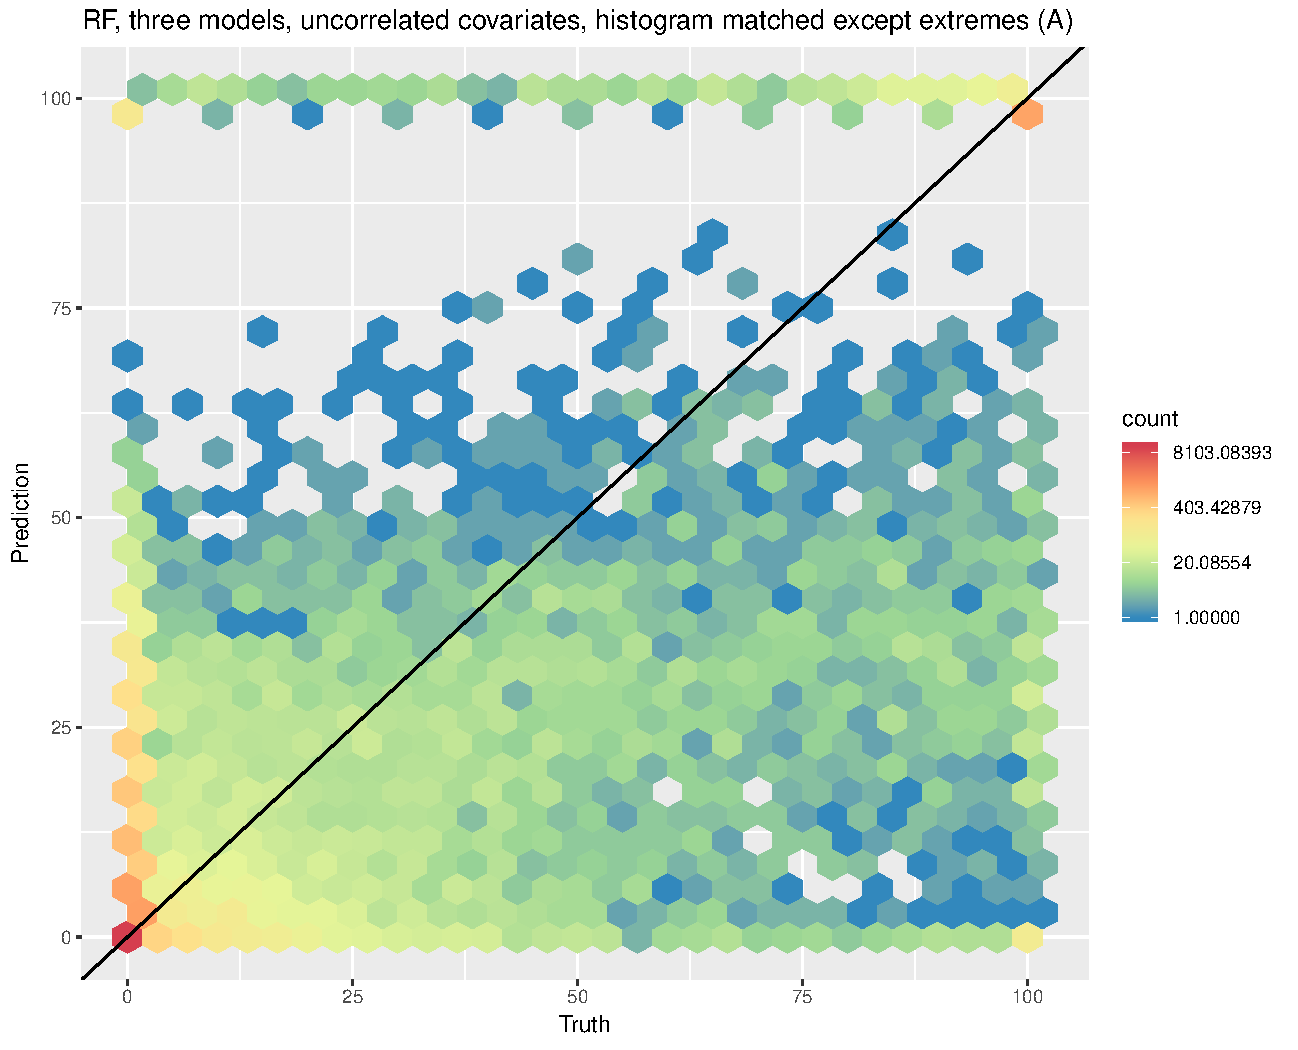
\includegraphics[width=0.8\textwidth]{article-figures/hexplots/2019-03-22-rf-3m-uncor-hma-hex}
    \caption{Random Forest three-step model prediction (histogram matched middle, proportionally) correspondence to ground truth.}
    \label{hex-rf-3m-uncor-hma}
\end{figure}
\begin{figure}
    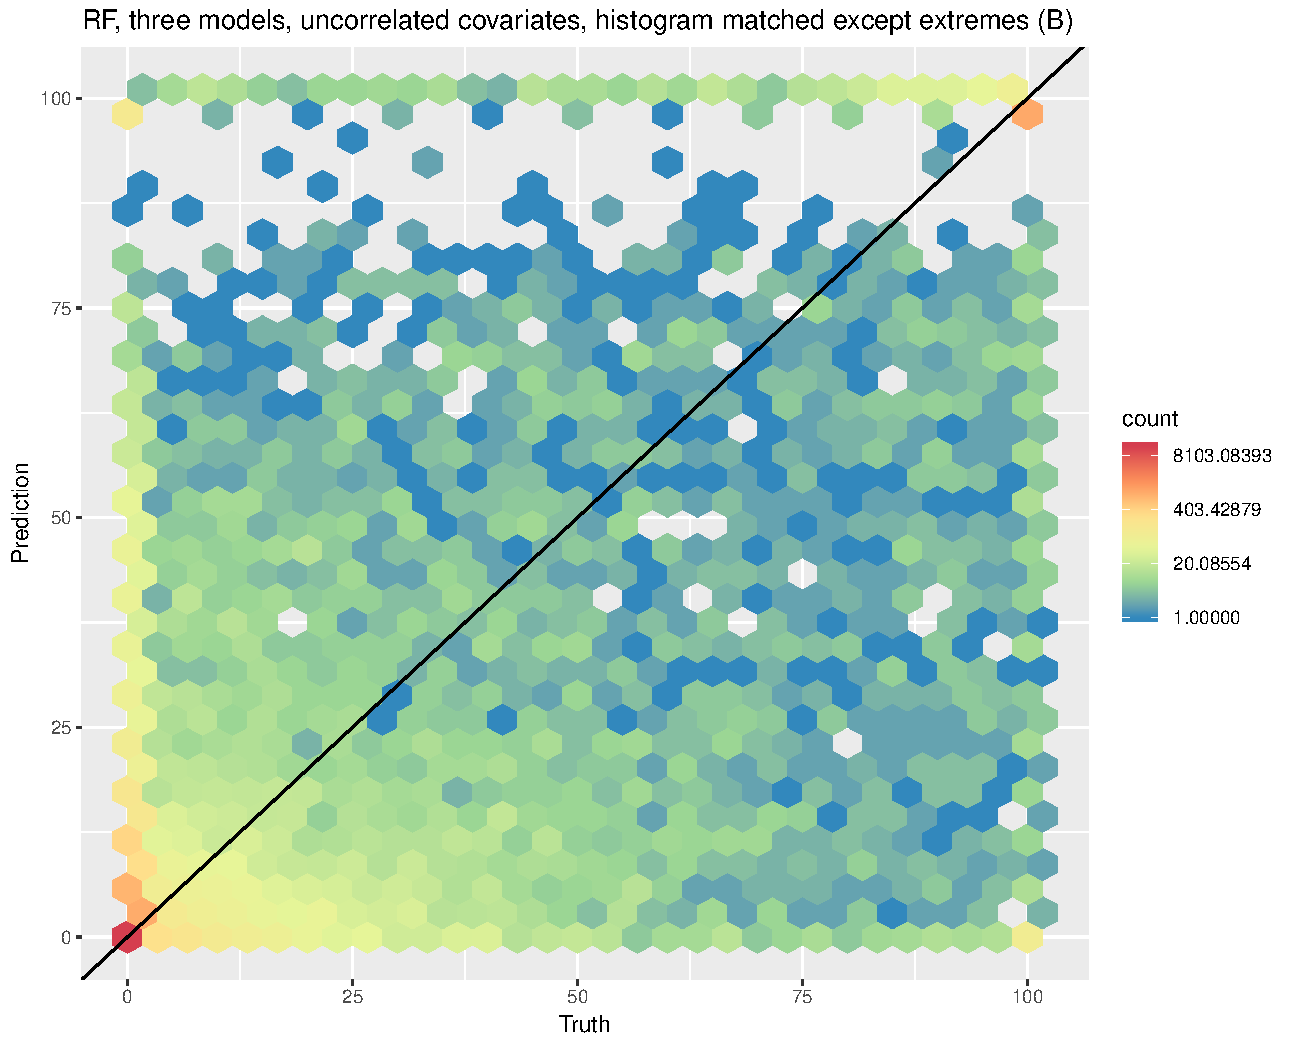
\includegraphics[width=0.8\textwidth]{article-figures/hexplots/2019-03-22-rf-3m-uncor-hmb-hex}
    \caption{Random Forest three-step model prediction (histogram matched non-extremes) correspondence to ground truth.}
    \label{hex-rf-3m-uncor-hmb}
\end{figure}

% Boxplots
\begin{figure}
    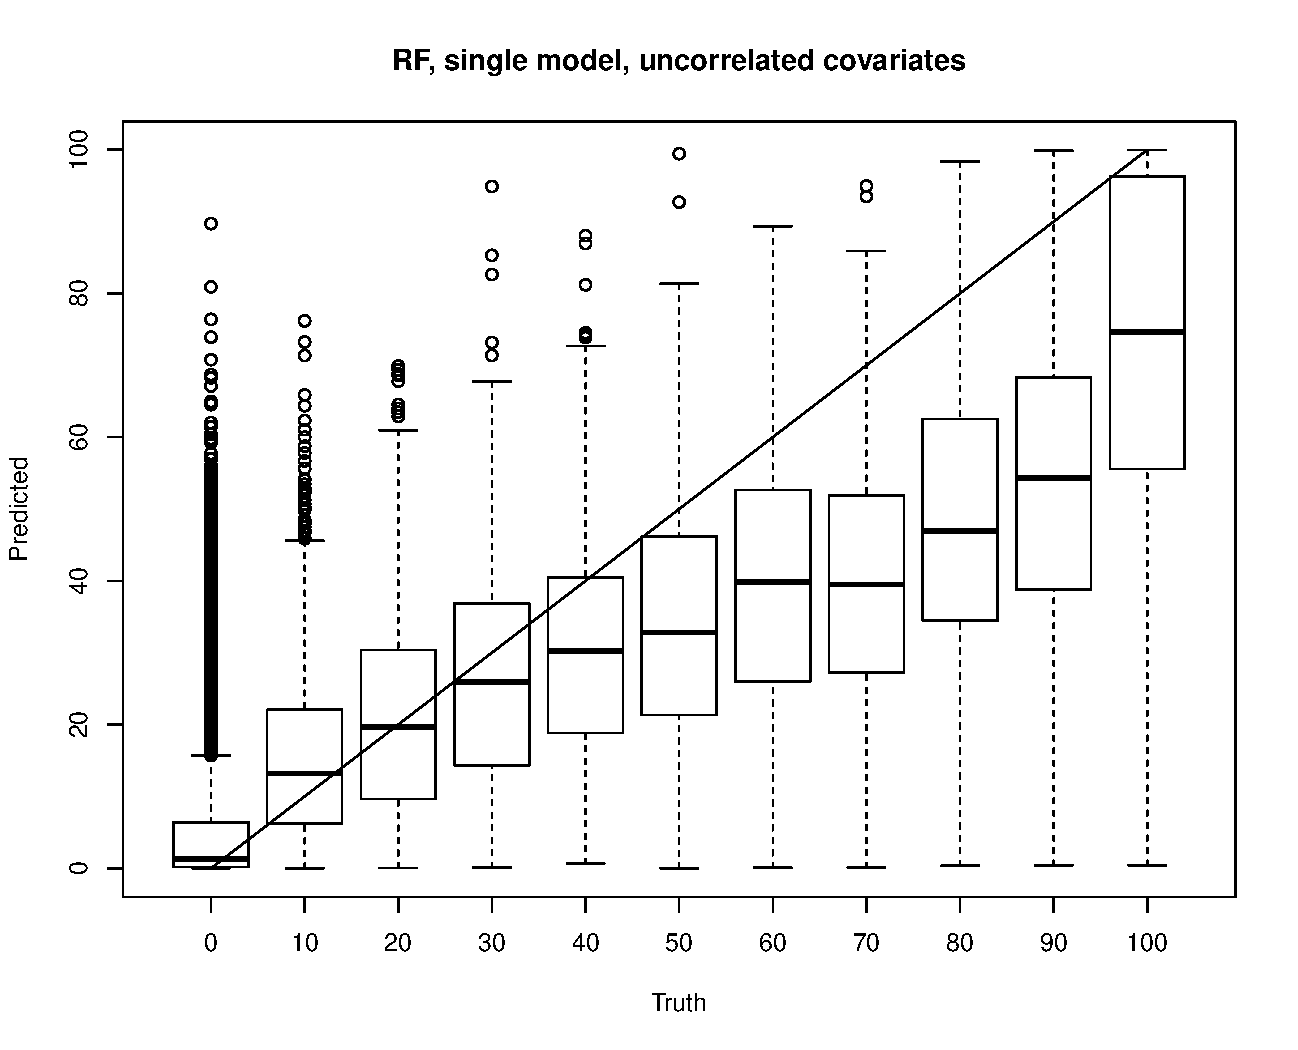
\includegraphics[width=0.8\textwidth]{article-figures/boxplots/2019-03-19-rf-1m-uncor-box}
    \caption{Random Forest single model prediction correspondence to ground truth.}
    \label{box-rf-1m-uncor-hm}
\end{figure}
\begin{figure}
    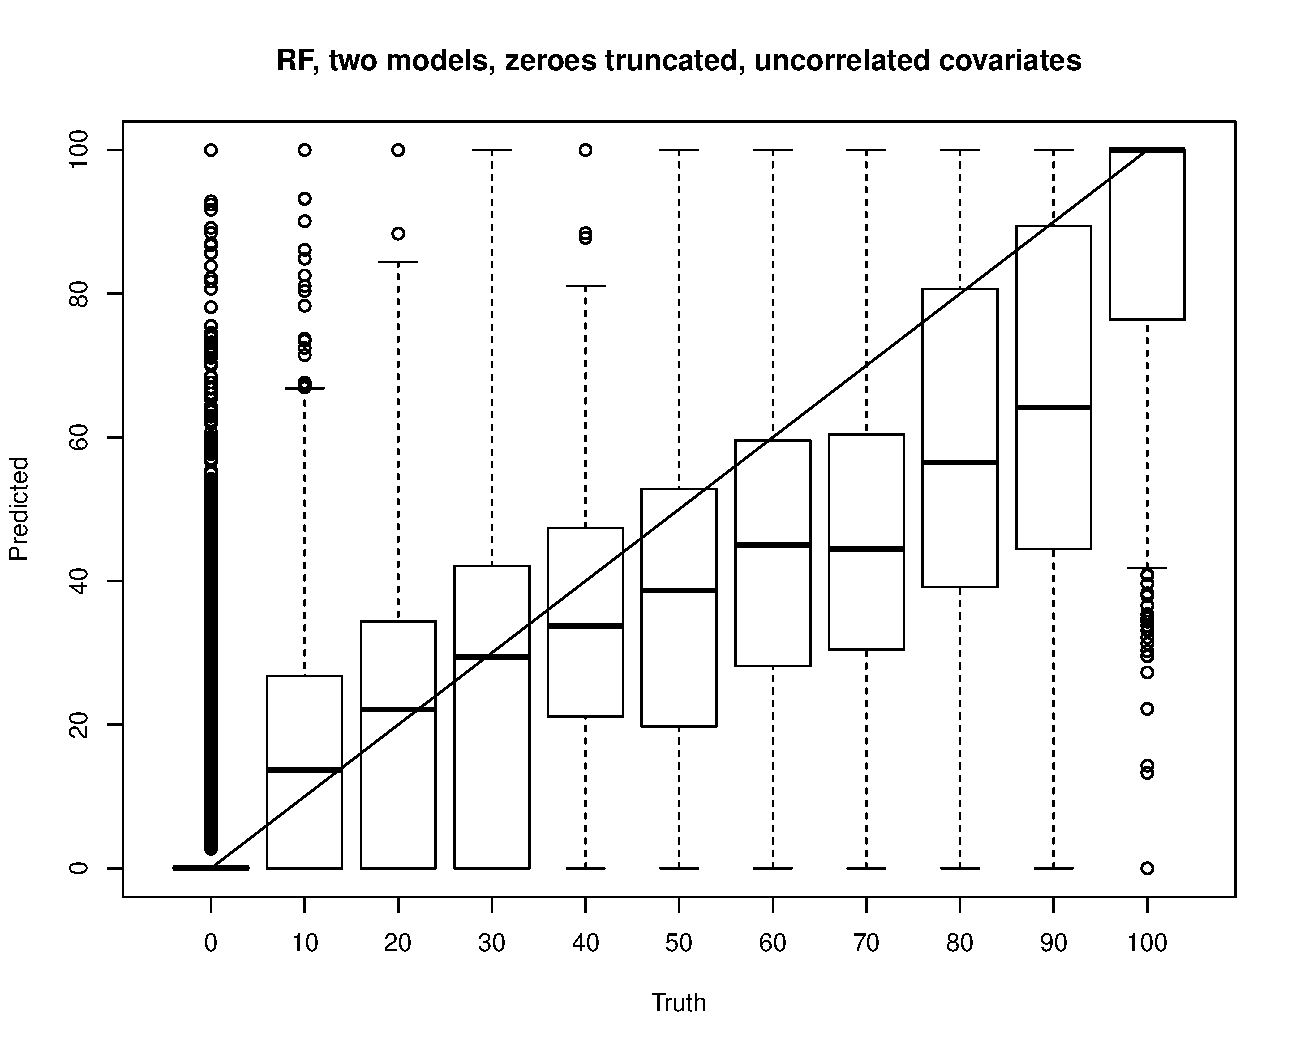
\includegraphics[width=0.8\textwidth]{article-figures/boxplots/2019-03-19-rf-2m-uncor-box}
    \caption{Random Forest two-step model prediction correspondence to ground truth.}
    \label{box-rf-2m-uncor-hm}
\end{figure}
\begin{figure}
    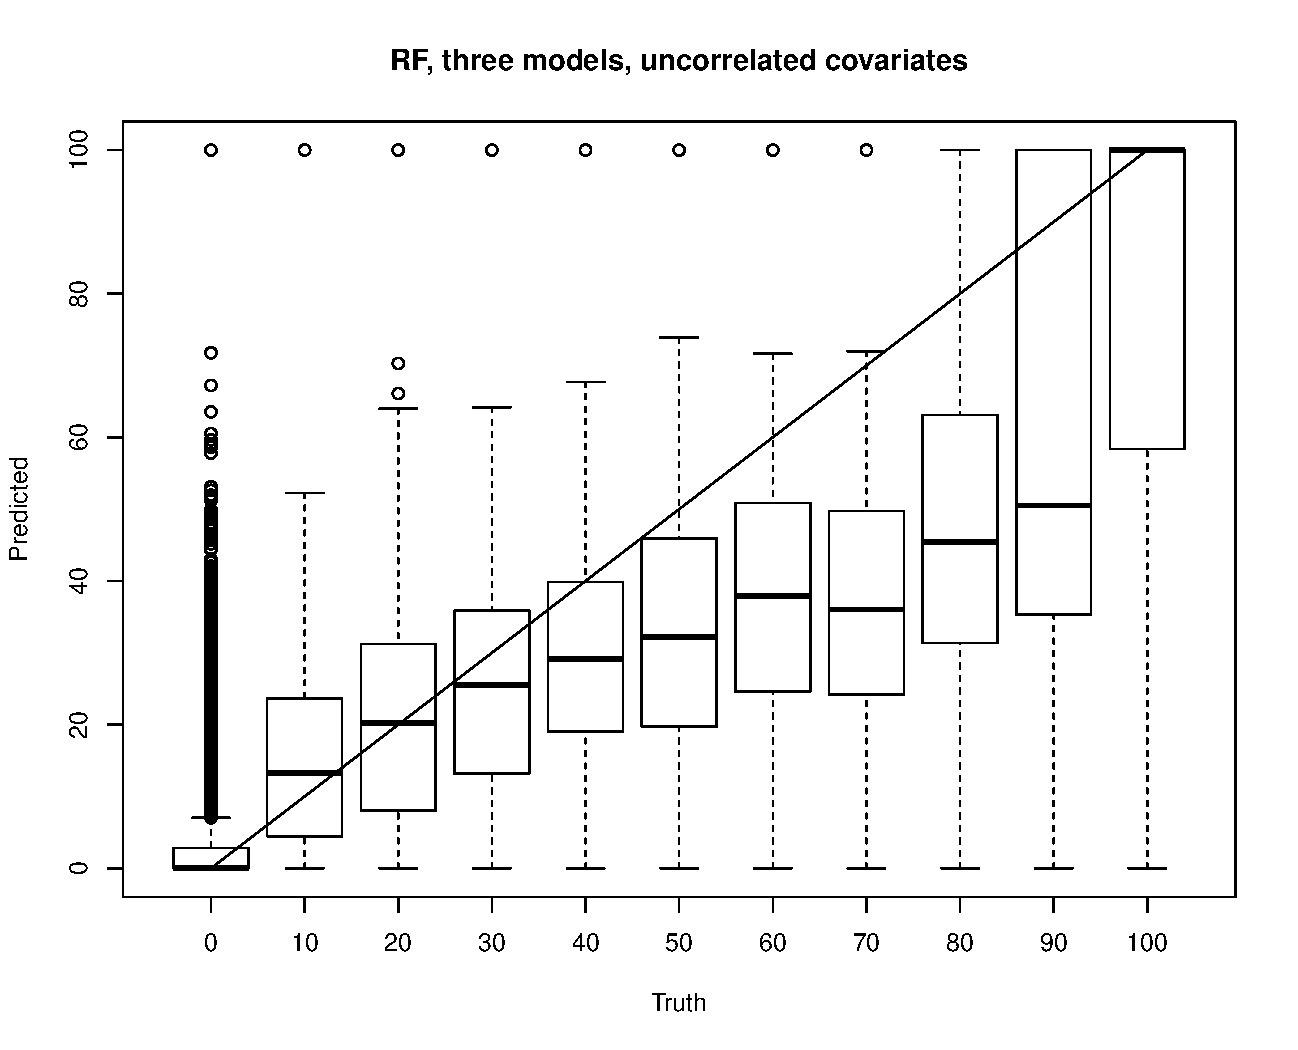
\includegraphics[width=0.8\textwidth]{article-figures/boxplots/2019-03-19-rf-3m-uncor-box}
    \caption{Random Forest three-step model prediction correspondence to ground truth.}
    \label{box-rf-3m-uncor-hm}
\end{figure}

% Barplots
\begin{figure}
    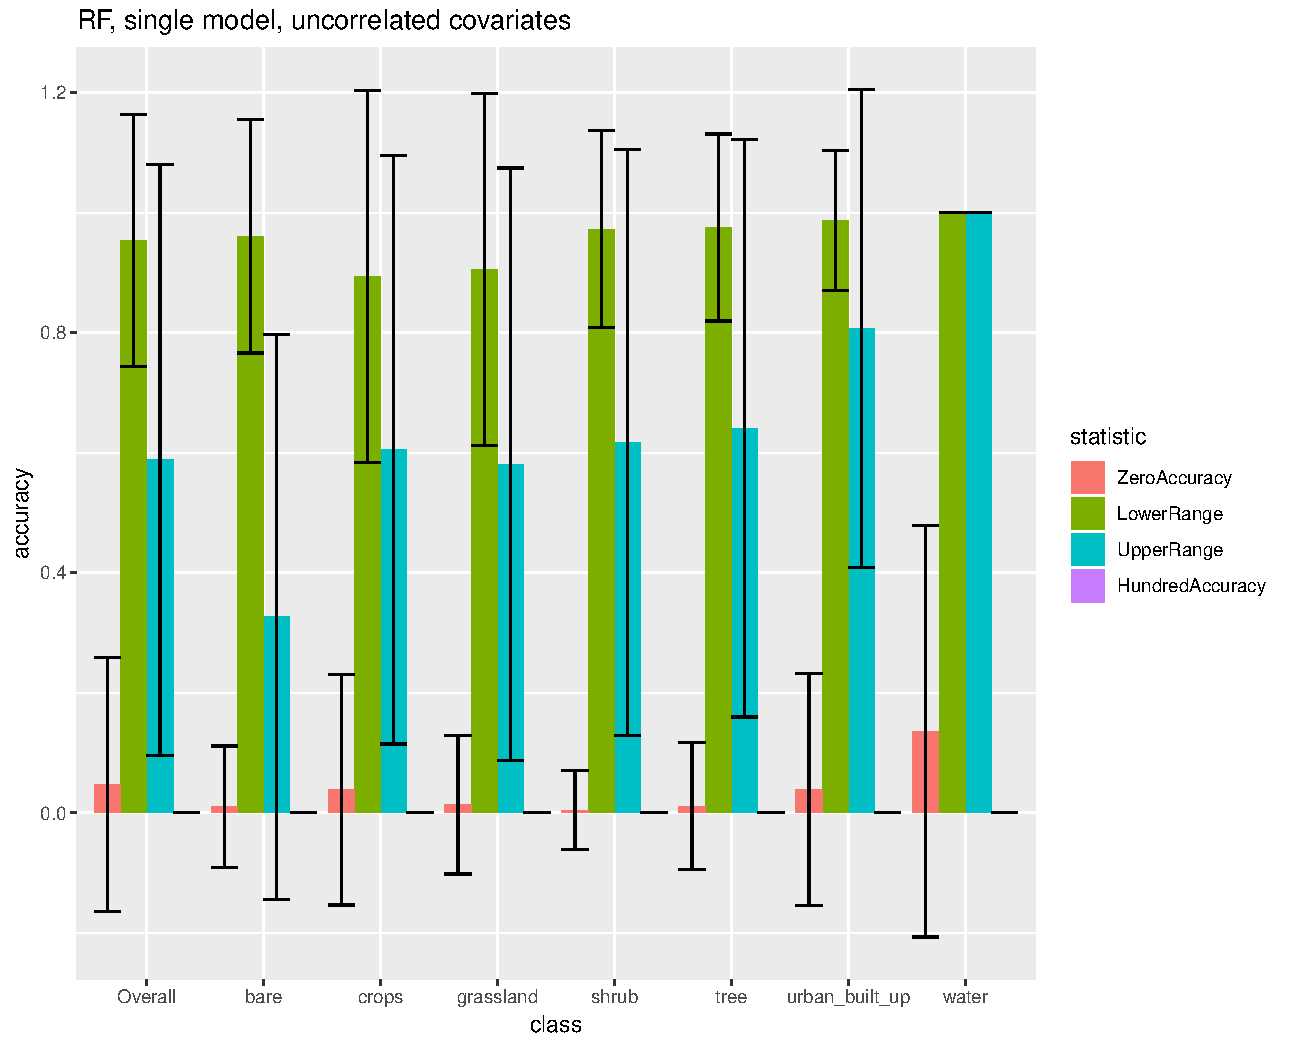
\includegraphics[width=0.8\textwidth]{article-figures/barplots/2019-03-19-rf-1m-uncor-bar}
    \caption{Random Forest single model prediction accuracies per class, per predicted magnitude (extremes vs middle)}
    \label{bar-rf-1m-uncor}
\end{figure}
\begin{figure}
    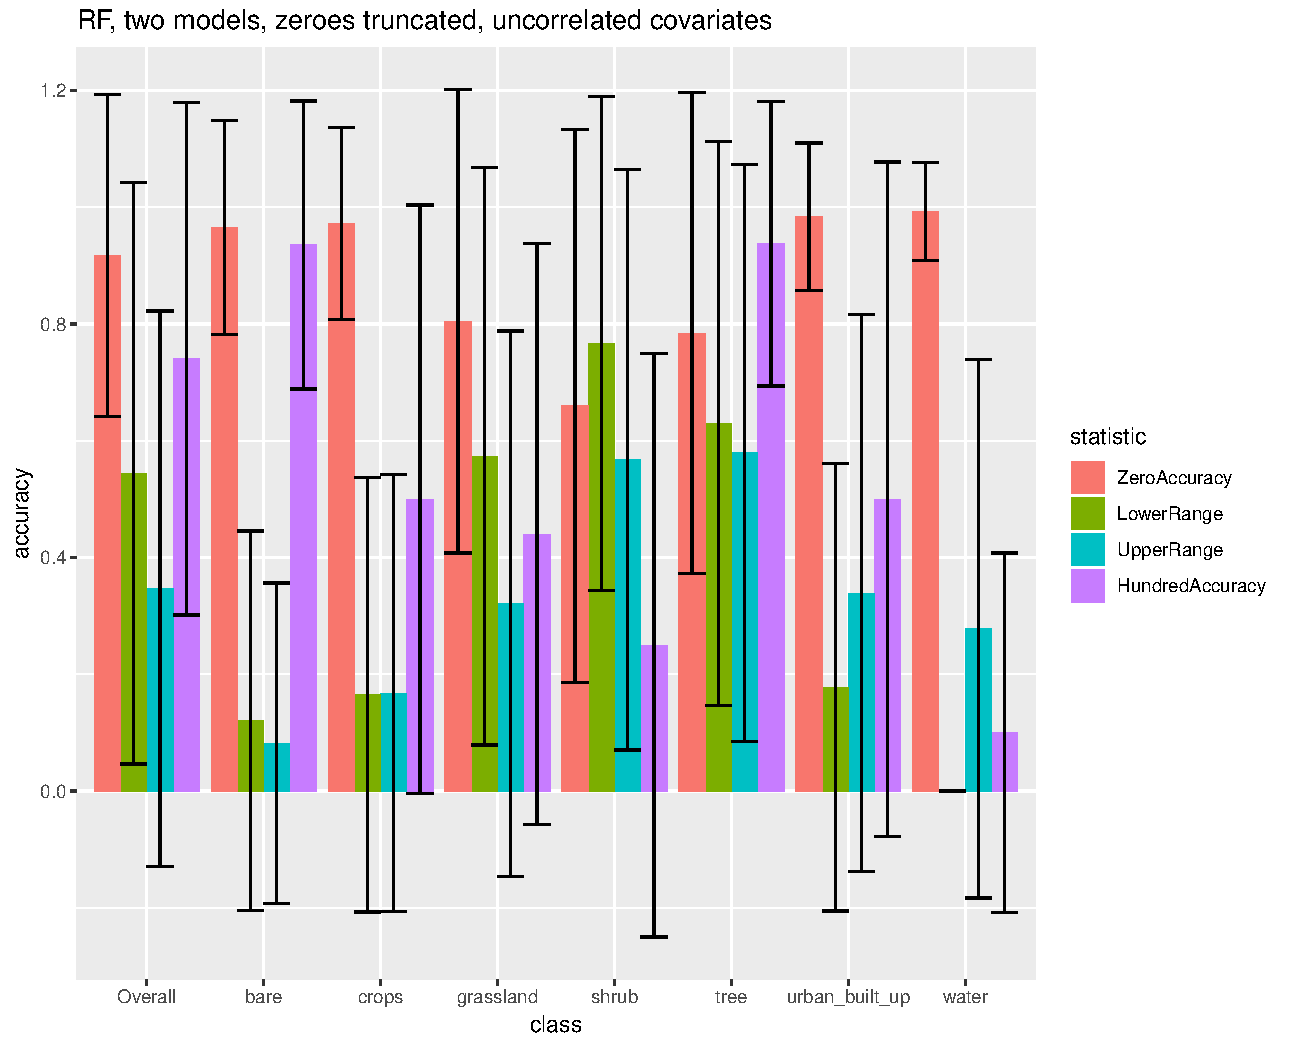
\includegraphics[width=0.8\textwidth]{article-figures/barplots/2019-03-19-rf-2m-uncor-bar}
    \caption{Random Forest two-step model prediction accuracies per class, per predicted magnitude (extremes vs middle)}
    \label{bar-rf-2m-uncor}
\end{figure}
\begin{figure}
    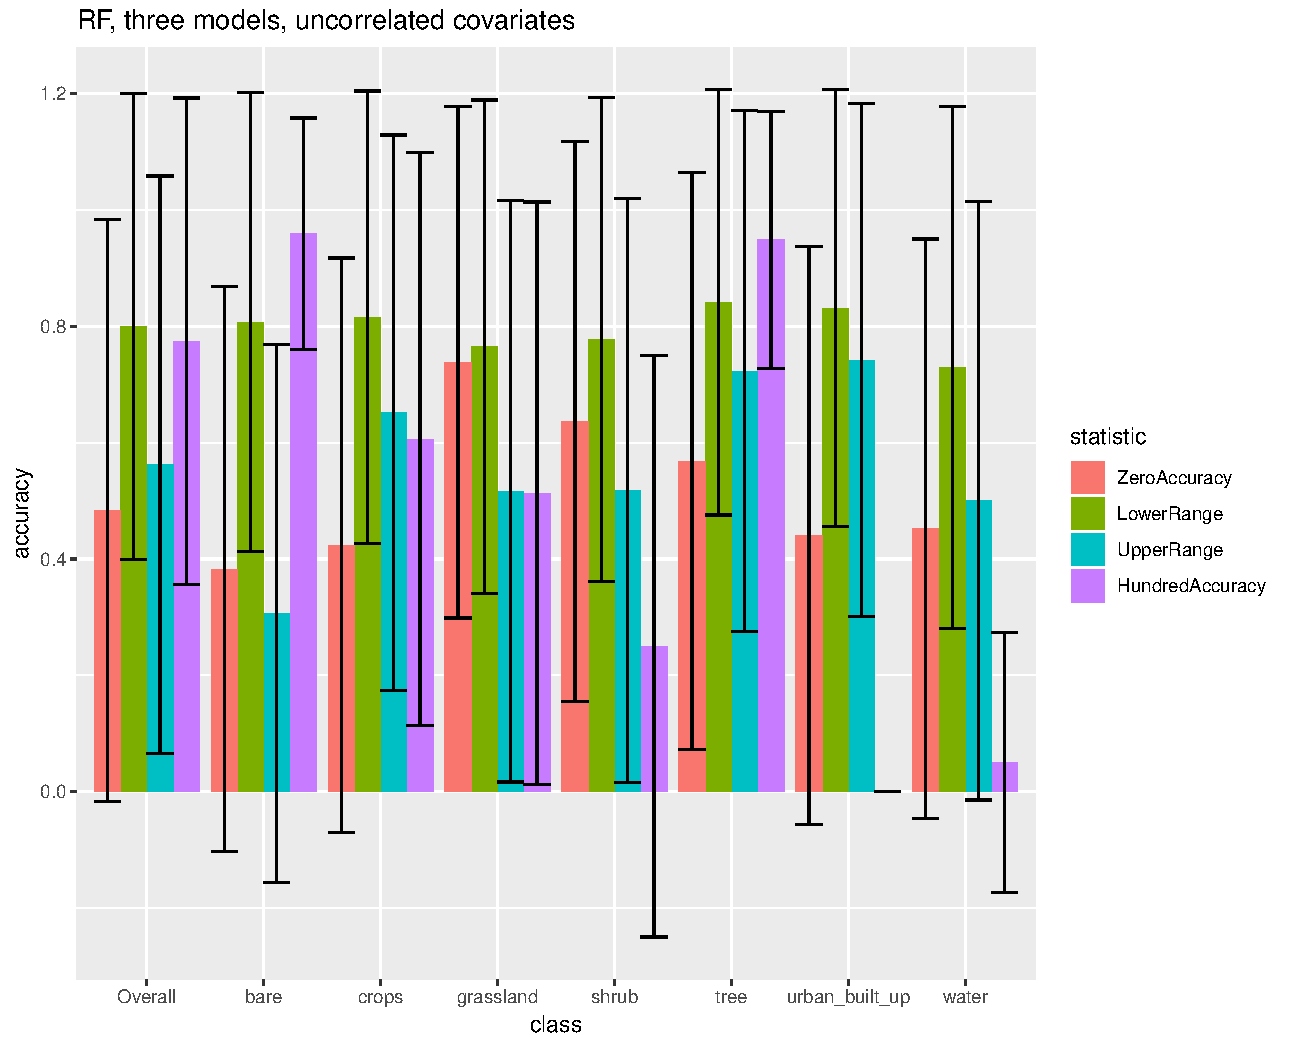
\includegraphics[width=0.8\textwidth]{article-figures/barplots/2019-03-19-rf-3m-uncor-bar}
    \caption{Random Forest three-step model prediction accuracies per class, per predicted magnitude (extremes vs middle)}
    \label{bar-rf-3m-uncor}
\end{figure}
\begin{figure}
    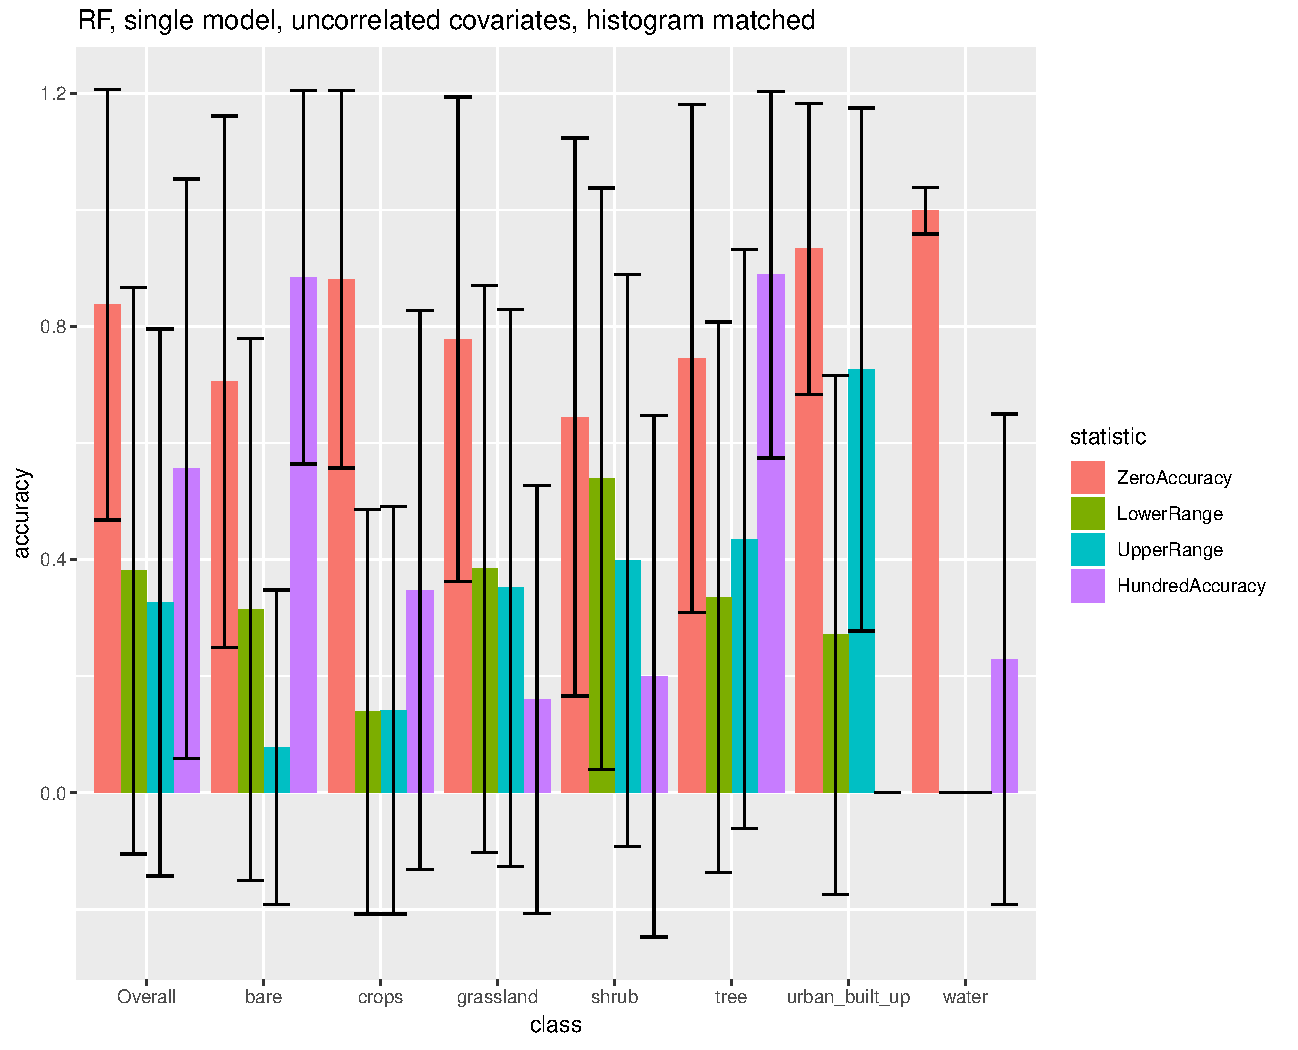
\includegraphics[width=0.8\textwidth]{article-figures/barplots/2019-03-22-rf-1m-uncor-hm-bar}
    \caption{Random Forest single model prediction (histogram matched) accuracies per class, per predicted magnitude (extremes vs middle)}
    \label{bar-rf-1m-uncor-hm}
\end{figure}
\begin{figure}
    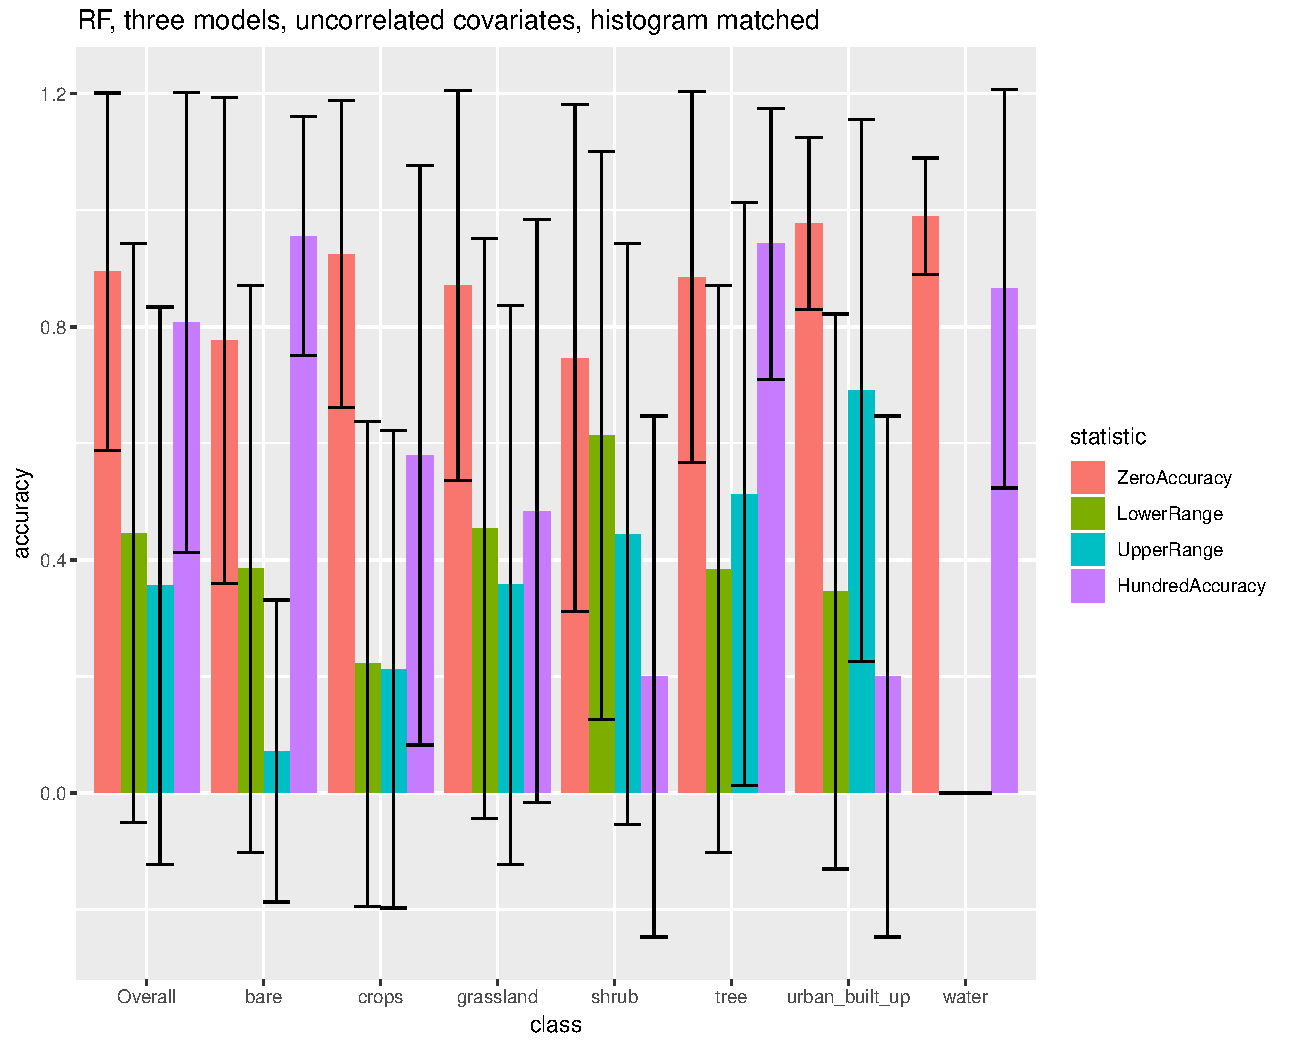
\includegraphics[width=0.8\textwidth]{article-figures/barplots/2019-03-22-rf-3m-uncor-hm-bar}
    \caption{Random Forest three-step model prediction (histogram matched) accuracies per class, per predicted magnitude (extremes vs middle)}
    \label{bar-rf-3m-uncor-hm}
\end{figure}

% Maps
\begin{figure}
    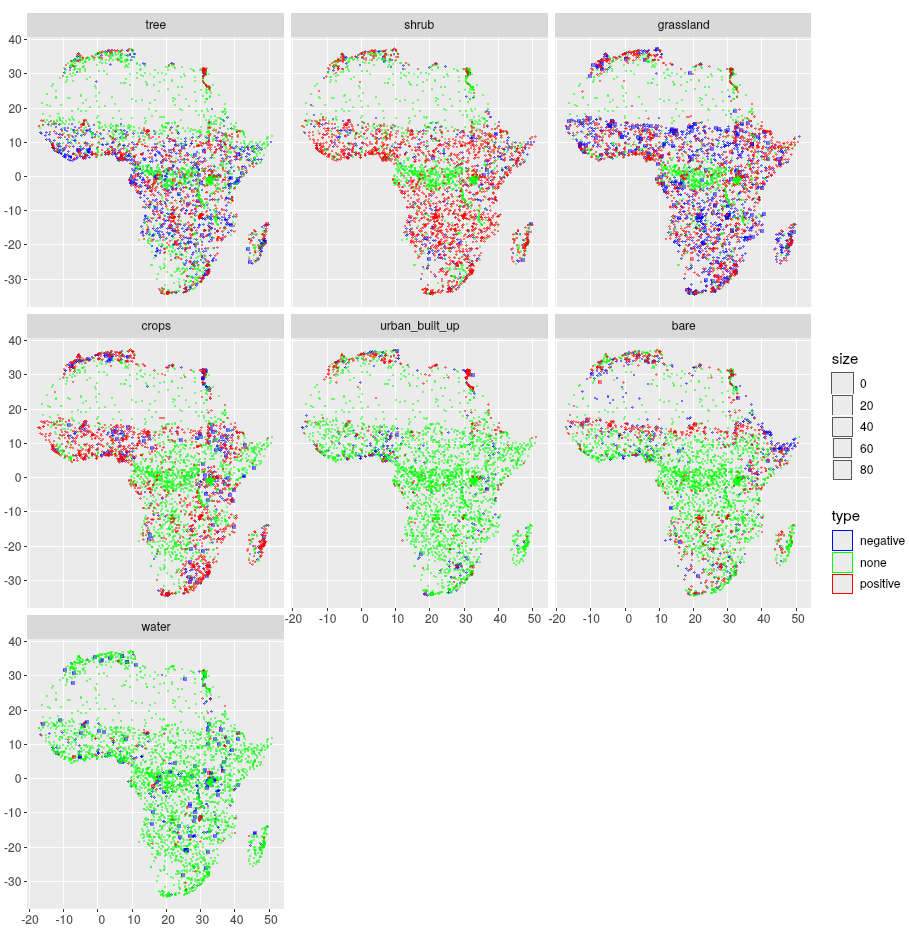
\includegraphics[width=\textwidth]{article-figures/maps/2019-03-26-rf-1m-bubble}
    \caption{Random Forest single model prediction residuals per class, spatially}
    \label{resid-rf-1m-uncor}
\end{figure}
\begin{figure}
    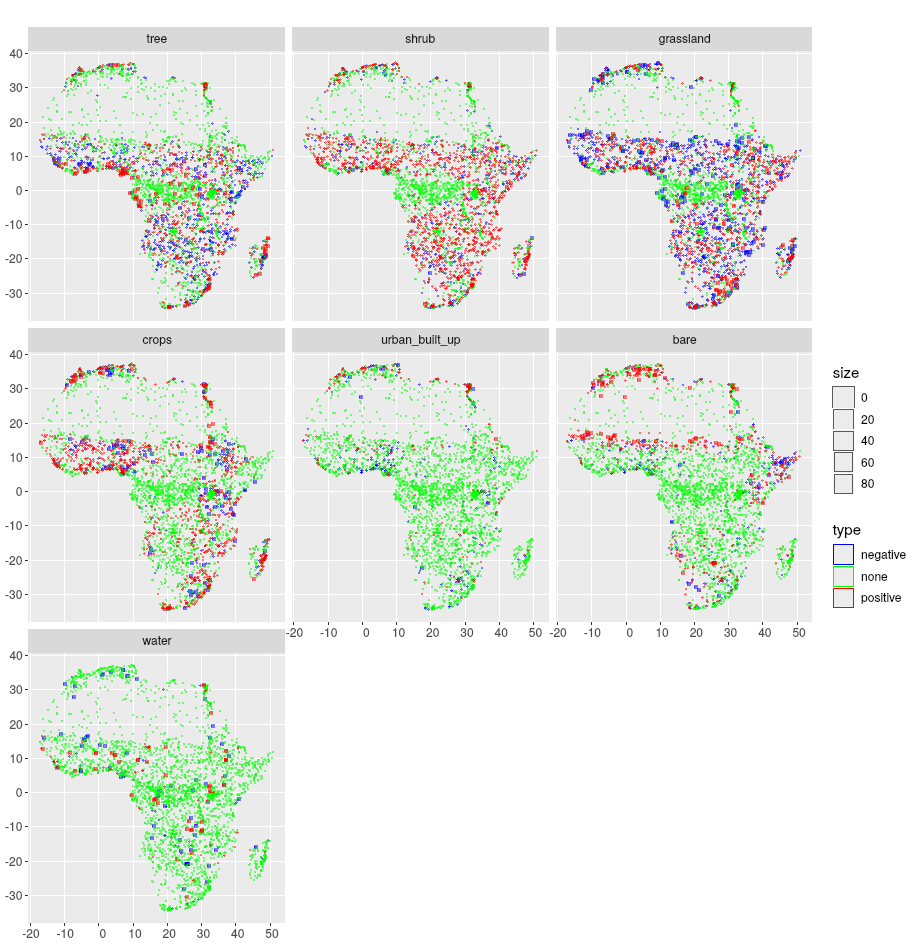
\includegraphics[width=\textwidth]{article-figures/maps/2019-03-26-rf-3m-bubble}
    \caption{Random Forest three-step model prediction residuals per class, spatially}
    \label{resid-rf-3m-uncor}
\end{figure}
\begin{figure}
    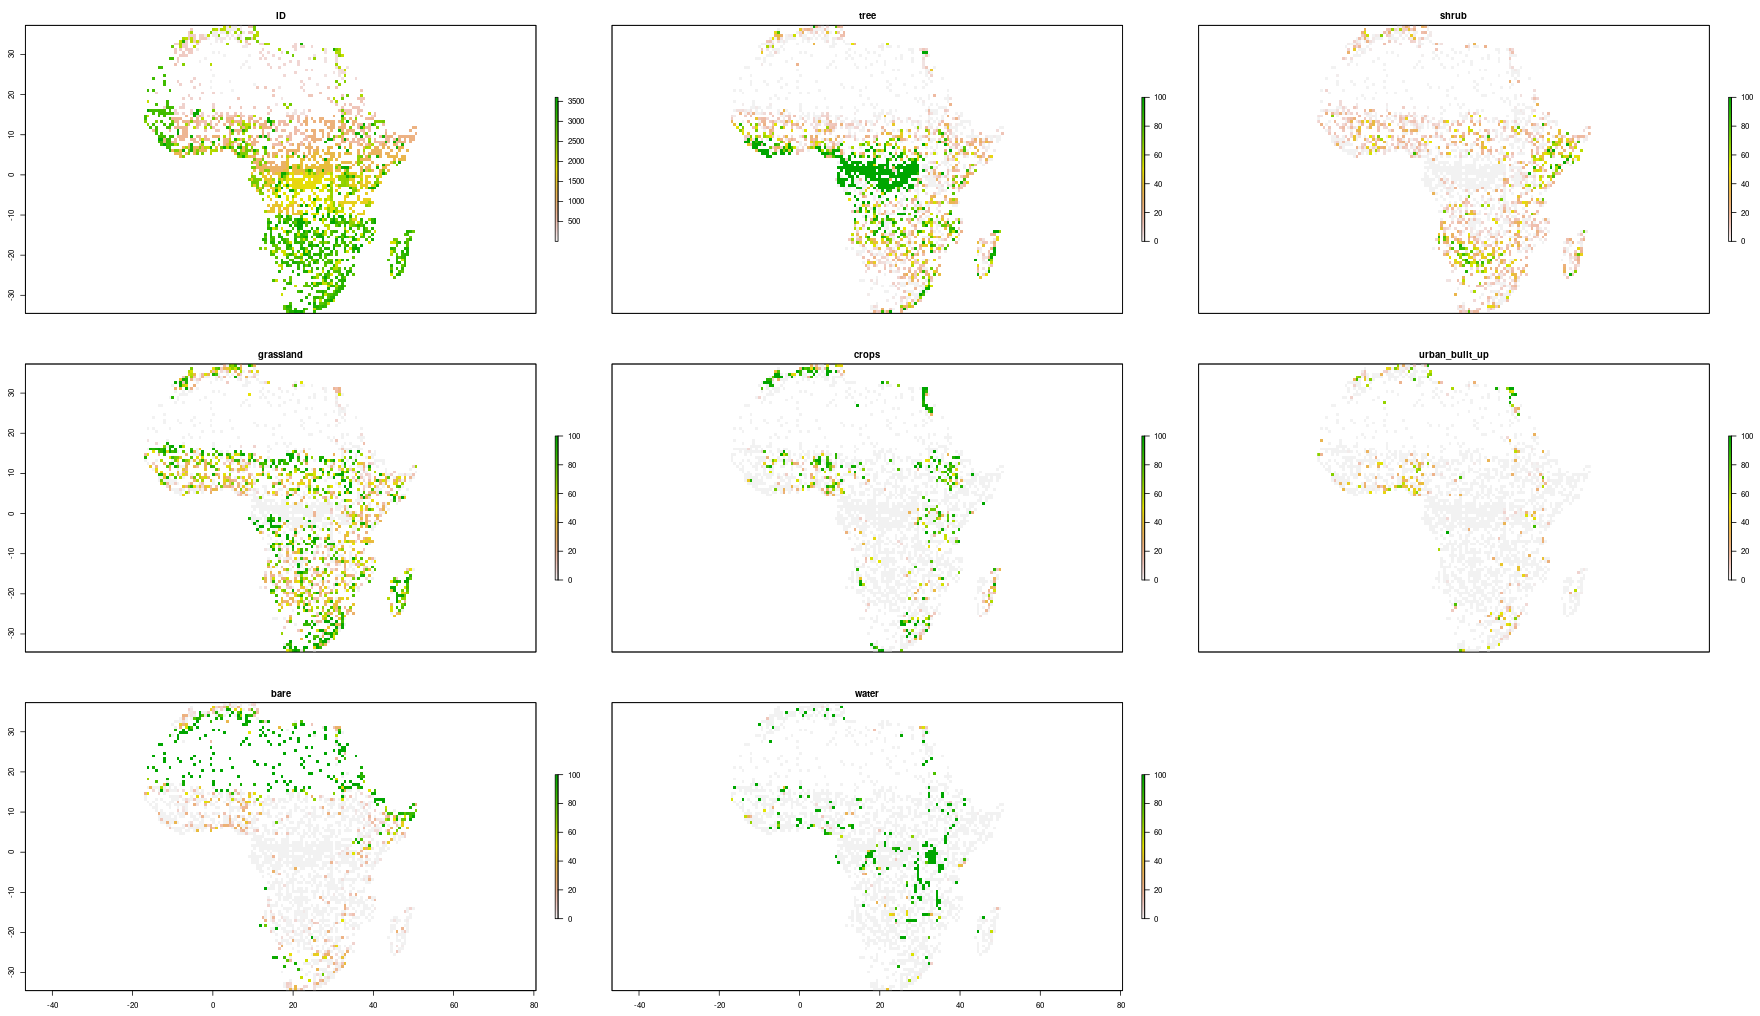
\includegraphics[width=\textwidth]{article-figures/maps/2019-04-10-rasterised-validation}
    \caption{Validation data spatially}
    \label{raster-validation}
\end{figure}
\begin{figure}
    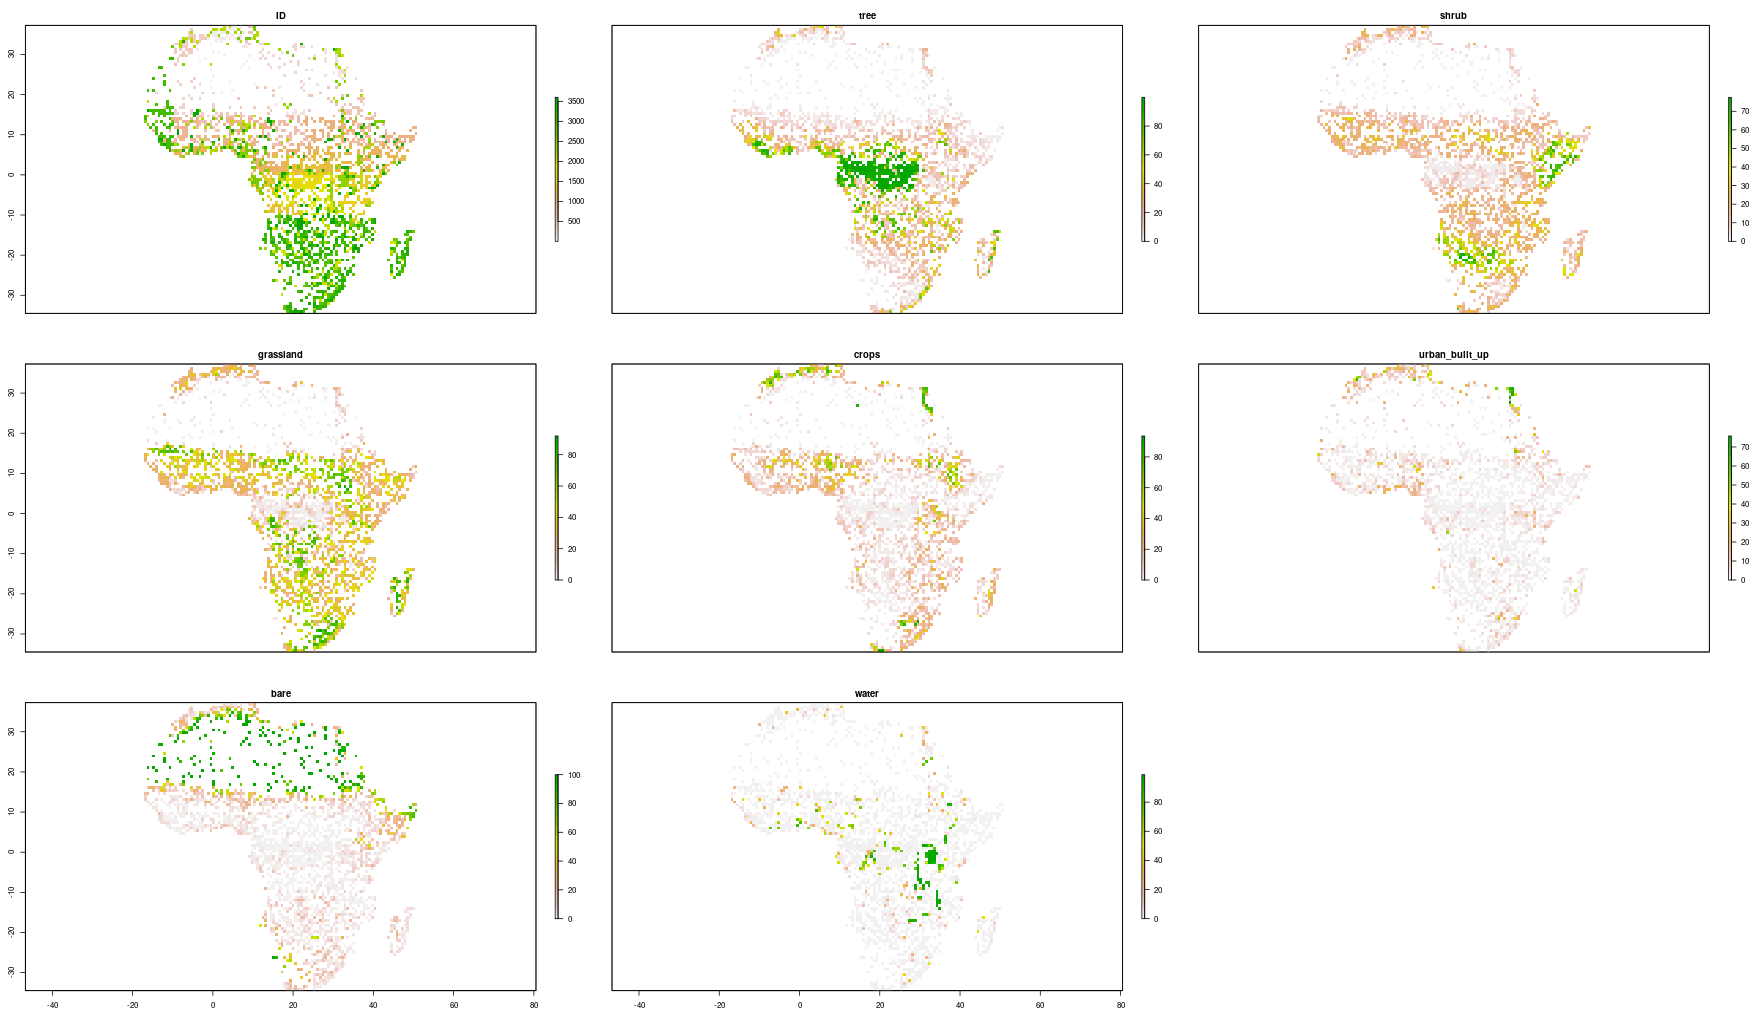
\includegraphics[width=\textwidth]{article-figures/maps/2019-04-10-rasterised-rf-1m-uncor}
    \caption{Random Forest single model predictions spatially}
    \label{raster-rf-1m-uncor}
\end{figure}

\section{Discussion}

\begin{enumerate}
 \item Fraction area accuracy goes up to 72\%, that is good considering that hard classification is not much better than that
 \item RF is the best, even though one model per class means that it does not take everything into account
 \item Accuracy assessment metric makes a big difference, useful to use subpixel confusion matrix for that
 \item Hardest to classify are grasslands and especially shrubs and urban
 \item All covariates are important to a certain degree (show table of importances)
 \item Histogram matching doesn't help any
\end{enumerate}

\section{Conclusions}

\begin{enumerate}
 \item Random forest is the best by some margin
 \item Subpixel confusion matrix is useful for differentiation
 \item All covariates are important but to a different degree
 \item Using a multi-model approach improves MAE at the cost of RMSE, thus a trade-off
\end{enumerate}

\minisection{Author Contributions} DM JV NT MH ML BK

\minisection{Funding} JRC CGLOPS

\minisection{Acknowledgements} VITO, time series group (BB)

\minisection{Conflicts of Interest} The authors declare no conflict of interest.

%\section*{Abbreviations}

\printnoidxglossary[type=acronym]

\bibliography{article-bib}

\end{document}
